% concatenated from Paper_2.2.tex
\documentclass[12pt]{amsart}

\usepackage[english]{babel}

% Set page size and margins
%\usepackage[left=2cm, right=5cm, top=2cm]{geometry}
\usepackage[a4paper]{geometry}
\usepackage{mathalfa}
\usepackage{tikz} 
\usepackage{caption}
\usepackage{subcaption}
% Useful packages
\usepackage{amsmath,amssymb,amsfonts,amsthm,a4,fleqn,bbm,dsfont,enumerate}
\usepackage{enumitem,cite}
%\usepackage[scr]{rsfso}
%\usepackage[utf8]{inputenc}
\textwidth=423pt \evensidemargin=9pt \oddsidemargin=9pt
\marginparsep=8pt \marginparpush=8pt \textheight=620pt
\topmargin=-20pt

\newtheorem{definition}{Definition}[section] 
\newtheorem{lemma}[definition]{Lemma}
\newtheorem{example}[definition]{Example}
\newtheorem{theorem}[definition]{Theorem}
\newtheorem{proposition}[definition]{Proposition}
\newtheorem{corollary}[definition]{Corollary}
\newtheorem{remark}[definition]{Remark}
\newtheorem{conjecture}[definition]{Conjecture}

\usepackage{graphicx}
\graphicspath{C:\Users\akhil\OneDrive\Desktop\Library Mathematics\Other}
\usepackage[colorlinks=true, allcolors=blue]{hyperref}
\makeatletter
\newcommand{\ostar}{\mathbin{\mathpalette\make@circled*}}
\newcommand{\make@circled}[2]{
	\ooalign{$\m@th#1\smallbigcirc{#1}$\cr\hidewidth$\m@th#1#2$\hidewidth\cr}
}
\newcommand{\smallbigcirc}[1]{
	\vcenter{\hbox{\scalebox{0.77778}{$\m@th#1\bigcirc$}}}
}
\@namedef{subjclassname@2020}{
	\textup{2020} Mathematics Subject Classification}
\makeatother

\begin{document}
	\title{Furtherness in finite topological spaces}
	\author[A. Badra]{Akhilesh Badra}
	\address{AKHILESH BADRA; Department of Mathematics, University of Delhi,
		Delhi--110 007, India}
	\email{akhileshbadra028@gmail.com}
	\author[H. K. Singh]{Hemant kumar Singh}
	\address{HEMANT KUMAR SINGH; Department of Mathematics, University of Delhi,
		Delhi--110 007, India}
	\email{hemantksingh@maths.du.ac.in}
	\thanks{The first author is supported by research grant from the Council of Scientific and Industrial Research (CSIR), Ministry of Science and Technology, Government of India with reference number: 09/0045(13774)/2022-EMR-I}
	
	\subjclass[2020]{Primary 54F65; Secondary 54E99}
	\keywords{ Finite topological space, Asymmetric metric space, Combinatorics}
	
	
	
	
	
	\maketitle
	\begin{abstract}
		In this paper, we introduce a novel distance-like notion of furtherness for finite topological spaces, demonstrating that every finite space can be viewed as an asymmetric pseudometric space. In particular, we show that every finite $T_0$ space is asymmetric metric space. The topology induced by the forward balls coincides with the original topology of the space, while the backward balls induce the opposite topology. To capture essential information about each finite space, we construct a furtherness Matrix, which gives significant structural details of the finite space. As an application, we introduce the notion of center and radius of subsets of finite topological spaces.
		
		
		
	\end{abstract}
	
	
	
	\section{\textbf{Introduction}}
	
	In metric spaces, the concept of distance provides a fundamental framework for analyzing the relationships between points. However, this notion is not universally applicable in arbitrary topological spaces. A subclass of topological spaces, known as metrizable spaces, allows the definition of distance between points through the existence of a compatible metric. Among finite spaces, only discrete spaces are metrizable, while non-discrete finite spaces inherently lack this property.  
	
	Given the practical utility and simplicity of finite spaces, which find applications across various domains, we propose a distance-like concept, termed "furtherness," defined for all finite spaces. Although this notion of furtherness is  not symmetric, but satisfies the properties of an asymmetric semidistance.
	%This furtherness measure, while not symmetric, serves as an asymmetric semidistance, offering a novel perspective on quantifying separation in finite spaces.
	%This paper introduces the notion of furtherness for finite topological spaces. 
	%This concept also extends our understanding of finite $T_0$ spaces by establishing them as asymmetric metric spaces.
	 We demonstrate that the topologies generated by forward and backward balls align with the original topology and its opposite, respectively. This provides a new lens to  interpret topological structures of finite spaces.\par 
	
	By the end of the $19^{th}$ century (Ref. \cite{Dedekind}), Richard Dedekind provided a characterization of modular lattices of finite length using what is now called a dimension function. The associated distance function reveals that every modular lattice of finite length can be viewed as an asymmetric metric space. In the begining of $20^{th}$ century (Ref. \cite{Birkhoff,Birkhoff2}), Garrett Birkhoff showed that the category of finite posets and the category of finite distributive lattices are essentially equivalent. Around the same time (Ref. \cite{Alexandroff}), Pavel Alexandroff established that finite $T_0$	spaces and finite posets are the same objects viewed from two different perspectives. Since every finite distributive lattice is a modular lattice of finite length, it follows that every finite $T_0$	space admits an associated asymmetric metric defined on it. Our notion of furtherness on finite spaces also verifies this result, particularly in the case of finite $T_0$	spaces. We show that every finite space can be regarded as an asymmetric pseudometric space. Using furtherness, one can prove that every finite $T_0$ space is an asymmetric metric space solely from the open sets of its topology, without any reliance to lattices or posets.\par
	
	Building upon the partial order structure inherent in finite spaces,  we establish a characterization of the preorder $x\leq y$ if and only if $x\in U_y$ (Ref. \cite{Stong}), % as introduced by R. E. Stong \cite{Stong},
	 within the framework of furtherness. This connection establishes a bridge between furtherness and fundamental concepts in algebraic topology,  offering new insights into the interplay between topological properties and distance-like notions in finite spaces.
	Central to this work is the construction of a furtherness matrix, which captures topological properties for each finite space. \par 
	

		We introduce the concepts of center and radius for subsets of finite topological spaces, which is parallel to the notion in metric spaces (Ref. \cite{Badra}). 
    	This work not only deepens the understanding of finite spaces through furtherness and partial order relations but also opens new pathways for exploring algebraic and topological properties in discrete settings.\par
	

	
	Throughout the paper, a finite space $X$ means a finite topological space.
	
	
	
	\section{\textbf{Furtherness function}}	\label{s2.1}
	
	
	In this section, we introduce a distance like notion of furtherness between any two points of a finite topological space. Let $X$ be a finite topological space with topology $\mathcal{T}$.
	%	Let $(X,\mathcal{T})$ be a finite topological space. and $A$ be a subset of X.  As $(X,\mathcal{T})$ is a finite topological space,
	So, the number of open sets in $\mathcal{T}$ will be finite. Therefore, for every $x\in X$, we can always get atleast one finite sequence of open sets such that $x\in U_0\subseteq U_1\subseteq U_2 \subseteq...\subseteq U_j\subseteq  ... \subseteq  X$.\par
	
	% such that $U_n\cap \partial_{X}(A)\neq\emptyset$. 
	Before moving on we first observe this in a few examples.
	
	\begin{example}\label{2.1}
		{\normalfont
			Let $X=\{1,2,3\}$ be a set and $\mathcal{T}=\{\emptyset,X,\{1,2\}\}$ be the topology on $X$.
			% Let $A=\{2,3\}\subseteq X$,
			Here, $1\in \{1,2\}\subseteq\{1,2,3\}=X$,  $2\in \{1,2\}\subseteq\{1,2,3\}=X$ and $3 \in\{1,2,3\}=X$.
		}
	\end{example}
	
	\begin{example}\label{2.2}
		{\normalfont
			Let $X=\{a,b,c,d\}$ be a set and $\mathcal{T}=\{\emptyset,X,\{a\},\{d\},\{a,b\},\{a,d\},\\ 
			\{a,b,d\}\}$ be the topology on $X$. %Let $A=\{2,3\}\subseteq X$, for $2\in A$, we have
			Here, $a\in\{a\}\subseteq \{a,b\}\subseteq\{a,b,d\}\subseteq\{a,b,c,d\}=X$, $b\in \{a,b\}\subseteq\{a,b,d\}\subseteq\{a,b,c,d\}=X$, $c\in\{a,b,c,d\}=X$ and $d\in\{d\}\subseteq \{a,d\}\subseteq\{a,b,c,d\}=X$.\par 
			In above examples, we can notice a finite sequence of open sets around every point of the space. But this sequence may not be unique around each point. In Example \ref{2.2}, for $a\in X$, we have $a\in\{a\}\subseteq \{a,d\}\subseteq\{a,b,d\}\subseteq\{a,b,c,d\}=X$, is another sequence around $a$.
		}
	\end{example}
	
	Given a finite space $X$ and $x\in X$, we have the minimal open set $U_x$, as the intersection of all the open sets which contains $x$ (Ref.   \cite{Barmak}).
	
	\begin{definition}
		Let $X$ be a finite space. A nested sequence of open sets around $x\in X$ is a sequence $(U_j)_{j\geq 0}$ of open subsets $U_j$ of $X$ such that  $U_0=U_x$ and $U_j\subset U_{j+1},$ and there is no open set between $U_j$ and $U_{j+1}$ for all $j\geq 0$, where $U_j\subset U_{j+1}$ means $U_j$ is properly contained in $U_{j+1}$.
	\end{definition}
	
	Now, with the help of these nested sequences of open sets around a point $x\in X$, we define a notion of furtherness from $x$ to any point $y$ of $X$.
	
	\begin{definition}
		Let $X$ be a finite space and $x,y\in X$. The furtherness of $x$ from $y$ is the smallest whole number $k$ such that there exist a nested sequence $(U_j)_{j\geq0}$ of open sets around $x$ such that $y\in U_k$.
	\end{definition}
	
	
	In a finite space $X$, we always have finite number of nested sequences of open sets $(U_j)_{j\geq 0}$ around $x\in X$. We denote these sequences by $(U^i_j)_{j\geq 0}$, where $1\leq i\leq m, \text{ and } m\in \mathbb{N}$. For every $y\in X$ and a finite sequence $(U^i_j)_{j\geq 0}$, let $k_i$ be the least number such that $y\in U^i_{k_{i}}$. We define a map $\Psi_x: X\longrightarrow \{0,1,2,...,|X|-1\}\subseteq\mathbb{N}\cup \{0\}$, such that $\Psi_x(y)=\min\{k_i|1\leq i\leq m\}$.  Thus, $\Psi_{x}(y)$ is the furtherness of $x$ from $y$. It is clear that $\Psi_x(y)$ is uniquely determined for every $y\in X$. \par 
	
	This motivates us to introduce the furtherness function for every finite space $X$. 
	
	\begin{definition}[Furtherness function]
		Let $X$ be a finite space. The furtherness function on $X$ is a function $\Psi:X\times X\longrightarrow \{0,1,2,...,|X|-1\}\subseteq\mathbb{R}$, such that $\Psi(x,y)=\Psi_{x}(y),\forall x,y\in X$.
	\end{definition}
	
	
	Notice that $x\in U_0$, for every nested sequence $(U_j)_{j\geq 0}$ around $x$. So, the furtherness of every point from itself is zero. That is, $\Psi(x,x)=\Psi_{x}(x)=0,\forall x\in X.$\\
	
	%A topology $\mathcal{T}$ on a finite set $X$ is a collection of its subspaces that satisfies certain axioms. We have this
	Using the  partial order relation $\leq$ on a topology $\mathcal{T}$ of $X$ such that $U\leq V$ if and only if $U\subseteq V,$ for $U,V\in \mathcal{T},$ we can associate a poset daigram of $X$. For example
	% For any $x\in X$, we can observe the nested sequences of open sets around $x$ in the associated poset diagram of $(X,\mathcal{T})$. 
	
	
	%\begin{tikzpicture}[main/.style ] 
	%	\node[main] (1) {$\{a,b,c,d\}$}; 
	%	\node[main] (2) [below right of=1] {$\{a,b,d\}$};
	%	\node[main] (3) [below left of=2] {$\{a,b\}$}; 
	%	\node[main] (4) [below right of=2] {$\{a,d\}$};
	%	\node[main] (5) [below left of=4] {$\{a\}$}; 
	%	\node[main] (6) [below right of=4] {$\{d\}$};
	%	\node[main] (7) [below left of=6] {$\emptyset$};
	%	\draw (2) -- (4);
	%		\draw (2) -- (3);
	%			\draw (1) -- (2);
	%				\draw (3) -- (5);
	%					\draw (4) -- (5);
	%						\draw (4) -- (6);
	%							\draw (5) -- (7);
	%								\draw (6) -- (7);
	%	\end{tikzpicture}

%\begin{tikzpicture}[main/.style = {draw, circle}] 
%	\node[main] (1) {$x_2$}; 
%	\node[main] (2) [above left of=1] {$x_1$};
%	\node[main] (3) [below left =2] {$x_3$}; 
%	\node[main] (4) [below right of=3] {$x_4$};
%	\node[main] (5) [below left of=3] {$x_5$}; 
%	\node[main] (6) [below right of=5] {$x_6$};

%\end{tikzpicture}

\begin{center}
	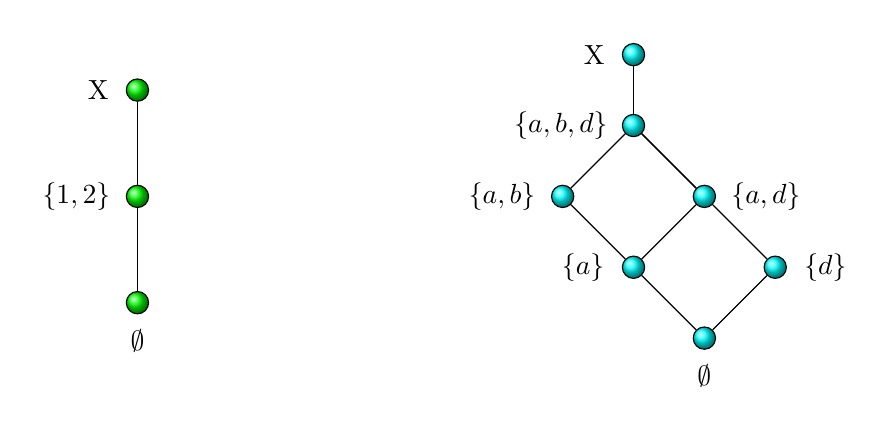
\begin{tikzpicture}  
		[scale=.9,auto=center,every node/.style={circle,fill=blue!10}] % here, node/.style is the style pre-defined, that will be the default layout of all the nodes. You can also create different forms for different nodes.  
		
		\node (a1) at (5,4.5) [ball color=green, circle, draw=black, inner sep=0.1cm, label=left:X] {};  
		\node (a2) at (5,3)  [ball color=green, circle, draw=black, inner sep=0.1cm, label=left:{$\{1 ,2\}$}]{}; % These all are the points where we want to locate the vertices. You can create your diagram first on a rough paper or graph paper; then, through the points, you can create the layout. Through the use of paper, it will be effortless for you to draw the diagram on Latex.  
		\node (a3) at (5,1.5) [ball color=green, circle, draw=black, inner sep=0.1cm, label=below :$\emptyset$]{};  
		%\node (F012) at (3,3) [label=left:{$\{x_2,\tau\} $}]  {};
		%	\node (a4) at (6,3)   [label=right: $ ; $]{};  
		%	\node (a5) at (5,2) [label=left:$\{a\}$] {};  
		%	\node (a6) at (7,2)  [label=right:$\{d\}$]{};  
		%	\node (a7) at (6,1) [label=below:$\emptyset$] {};   
		
		\draw (a1) -- (a2); % these are the straight lines from one vertex to another  
		\draw (a2) -- (a3);  
		%	\draw (a2) -- (a4);  
		%	\draw (a3) -- (a5);  
		%	\draw (a4) -- (a5);  
		%	\draw (a4) -- (a6);  
		%	\draw (a5) -- (a7);  
		%	\draw (a6) -- (a7);  
		
		\tikzstyle{point1}=[ball color=cyan, circle, draw=black, inner sep=0.1cm]
		\tikzstyle{point2}=[ball color=green, circle, draw=black, inner sep=0.1cm]
		\tikzstyle{point3}=[ball color=red, circle, draw=black, inner sep=0.1cm]
		
		
		\node (v1) at (12,5) [ball color=cyan, circle, draw=black, inner sep=0.1cm, label=left:X] {};
		\node (v2) at (12,4) [point1, label=left:{$\{a,b,d\}$}] {};
		\node (v3) at (11,3) [point1,label=left:{$\{a,b\}$}] {};
		\node (v4) at (13,3) [point1,label=right:{$\{a,d\}$}] {};
		\node (v5) at (12,2) [point1,label=left:$\{a\}$] {};
		\node (v6) at (14,2) [point1,label=right: $\{d\}$] {};
		\node (v7) at (13,1) [point1, label=below:$\emptyset$] {};
		
		\draw (v1) -- (v2);
		\draw (v2) -- (v3) -- (v5);
		\draw (v2) -- (v4) -- (v5);
		\draw (v2) -- (v4) -- (v6);
		\draw (v5) -- (v7);
		\draw (v6) -- (v7);
		
		%%\node (v8) at (intersection of v2--v3 and v5--v6) [point3] {};
		%	\node (v9) at (intersection of v2--v4 and v5--v7) [point3] {};
		%	\node (v10) at (intersection of v3--v4 and v6--v7) [point3] {};
		
		%	\draw (v3) -- (v8) -- (v6);
		%	\draw (v4) -- (v9) -- (v7);
		%	\draw (v4) -- (v10) -- (v7);
		%	\draw (v8) -- (v9) -- (v10);
	\end{tikzpicture}  
	
	
\end{center}

\hspace{20mm}	Example \ref{2.1}\hspace{45mm} Example \ref{2.2}\\


In Example \ref{2.2}, furtherness of $a$ from $b$ is 1. As there are two nested sequences $a\in U^1_0=\{a\}\subset U^1_1= \{a,b\}\subset U^1_2=\{a,b,d\}\subset U^1_3=X$, and $a\in U^2_0=\{a\}\subset U^2_1= \{a,d\}\subset U^2_2=\{a,b,d\}\subset U^2_3=X$, of open sets around $a$. Here, $b\in  U^1_1$ and $b\in U^2_2$. So, $k_1=1$ and $k_2=2$. Thus, $\Psi(a,b)=\Psi_{a}(b)=\min\{k_1,k_2\}=1.$
Similarly, we have $\Psi(a,c)=3$ and $\Psi(a,d)=1.$\par 
In the same example, we can also notice that furtherness of $b$ from $a$ is 0. As there is only one nested sequence $b\in U_0=\{a,b\}\subset U_1=\{a,b,d\}\subset U_2=X$ around $b$, and $a\in U_0$. Thus, $\Psi(b,a)=\Psi_{b}(a)=0$. Similarly, the furtherness of $c$  from $a,b$ $\&$ $d$ is 0. It is cleat that the furthrerness function is not symmetric. This example also shows that $\Psi(x,y)=0$ does not imply $x=y$.

%	\begin{remark}
	%		{\normalfont
		%			Above example shows that furthrerness function is not symmetric. That is $\Psi(x,y)$ may not be same as $\Psi(y,x)$ for $x,y\in X$. And, it also shows that $\Psi(x,y)=0$ does not imply $x=y$.
		%		}
	%	\end{remark}

\begin{theorem}\label{2.6}
	
	% topological space such that it satisfies the $T_0$ separation axiom.
	Let $X$ be a finite $T_0$ space. Then $ \Psi(x,y)=\Psi(y,x)=0 \iff x=y,$ for $ x,y\in X$.
	
\end{theorem} 

\begin{proof}
	%As $X$ is $T_0$, for every $x,y\in X$ there exist an open set containing one and only one of them. Let $x,y\in X$ such that $x\neq y$. 
	Let $x\neq y$. Now, $ \Psi(x,y)=0 \implies y\in U_x$ and $\Psi(y,x)=0 \implies x\in U_y$.
	%Let  $ x,y\in X$ such that  $ \Psi(x,y)=\Psi(y,x)=0$. As $\Psi(x,y)=0$, $y\in U_x = U_0$, for every finite nested sequence $(U_j)_{j\geq 0}$ around $x$. Similarly, as $\Psi(y,x)=0$, $x\in U_y = V_0$, for every finite nested sequence $(V_j)_{j\geq 0}$ around $y$. So,  $x,y\in U_x$ and $x,y\in U_y$.
	% Which means there does not exist an open set that contains one and only one of $x$ or $y$, a contradiction.
	This contradicts the fact that $X$ is $T_0$. So, $x=y$. Conversely, if $x=y$ then $\Psi(x,y)=\Psi(y,x)=0$.
\end{proof}



\begin{example}\label{2.7}
	{\normalfont
		If $X$ is a finite indiscrete space then the furtherness of every point is 0 from any other point. And if $X$ is a finite discrete space then the furtherness of every point is 1 from any other point. Thus, the furtherness function is a metric on finite discrete spaces.
		
		% That is,  $\Psi(x,y)=\left\{ 
		%	\begin{array}{11} 
			%		0, & \text{if }x=y \\
			%		1, & \text{if }x\neq y \\
			%	\end{array}  $.
	}
	
	
	%Let $(X,\mathcal{T})$ be a finite topological space, where $\mathcal{T}$ is the trivial topology on $X$. Then furtherness of every point is 0 from any other point. As for any $x\in X$, there is just one nested sequence of open sets around $x$, that is $x\in U_0=X.$ and every point of $X$ belongs to $U_0$. So, $\Psi(x,y)=0,\forall x,y\in X$. \par
	
	%Let $(X,\mathcal{T})$ be a finite topological space, where $\mathcal{T}$ is the discrete topology on $X$. Then furtherness of $x\in X$ from $y(\neq x)\in X$ is 1. As for any $x,y\in X$, the pair $\{x,y\}$ will always be there in $\mathcal{T}$, for all $x\neq y\in X$. So, every nested sequence of open sets around $x$ starts from $U^i_0=\{x\}$, which means $k_i\geq 1, \forall i,$ and there will be a sequence such that $y\in U^j_1=\{x,y\}\implies k_j=1$. Thus, $\Psi_{x}(y)=\min_i\{k_i\}=1$. So, $\Psi(x,y)=1,\forall x\neq y\in X$.\par 
	
	
\end{example}

If $\Psi(x,y)=0$, then $U_y\subseteq U_x$. This gives the following result.

\begin{theorem}\label{2}
	Let $X$ be a finite topological space $x\in X$. Then the smallest open set containing $x$ is $U_x=\{y\in X |\Psi(x,y)=0\}$. %=\cup\{U_y|\Psi(x,y)=0\}.$
\end{theorem}
By above theorem, we get that the singleton $\{a\}$ is open in a finite space $X$ $\iff$ $\Psi(a,b)\neq0,\forall~ b\in X\backslash\{a\}$.
%	\begin{proof}
	%	If $\Psi(x,y)=0$, then $U_y\subseteq U_x$. That implies $\cup\{U_y|\Psi(x,y)=0\}\subseteq U_x$. If $a\in U_x\implies \Psi(x,a)=0$ and $a\in U_a\subseteq \cup\{U_y|\Psi(x,y)=0\}$. So, $U_x\subseteq \cup\{U_y|\Psi(x,y)=0\}$. Thus, $U_x=\cup\{U_y|\Psi(x,y)=0\}$.
	%	\end{proof}


\begin{remark}{\normalfont
		Given a finite topological space $X$ and $x,y\in X$, let $U_{x,y}$ be the smallest open set containing $\{x,y\}$. % As $x\in U_{x,y}\implies U_{x}\subseteq U_{x,y}$ and $y\in U_{x,y}\implies U_{y}\subseteq U_{x,y}$. Therefore $U_{x} \cup U_{y} \subseteq U_{x,y}$. Also, $\{x,y\}\subseteq U_{x} \cup U_{y} \implies U_{x,y} \subseteq U_{x} \cup U_{y}$.
		It is easy to see that  $U_{x,y} = U_{x} \cup U_{y}$. 
		Similarly, for a subset $A$ of $X$, the smallest open set containing $A$ is $U_A= \bigcup\limits_{a\in A} U_a.$
	}
\end{remark}

Next, we observe that, if $\Psi(x,y)=k,$ for $x,y\in X$, then how open sets before $k^{th}$ term in nested sequence $(U_j)_{j\geq 0}$ around $x$ are related, and prove that its $k^{th}$ term is always  the same, whenever $y\in U_k$.

\begin{lemma}\label{2.8.}
	Let $X$ be a finite space and $(U_j)_{j\geq0}$ be a nested sequence of open sets around $x\in X$, then $U_j= U_{j-1}\cup U_a$, for some $a\in X\backslash U_{j-1}$.
\end{lemma}

\begin{proof}
	As $U_{j-1}\subset U_{j}$, let $a\in U_j\backslash U_{j-1}$. So, we get $U_a\subseteq U_j$, and $U_{j-1}\subset U_{j-1}\cup U_a \subseteq U_j$. By the definition of nested sequence of open sets, we get $U_{j}=(U_{j-1}\cup U_a)$.
	% As $U_{j-1}\cup U_a$ is an open subset between $U_{j-1}$ and $U_j$ and  $U_{j-1}\neq (U_{j-1}\cup U_a)$, so $U_{j}=(U_{j-1}\cup U_a)$.
\end{proof}

It is easy to observe that, for an open subset $A$ of a finite  space $X$ such that $U_x\subseteq A$ for some $x\in X$, there exists a nested sequence $(U_j)_{j\geq 0}$ of open subsets around $x$ such that $U_k= A$ for $k\in \mathbb{N}\cup \{0\}$. 


\begin{theorem}\label{2.9.}
	Let $X$ be a finite space and $x,y\in X$ such that $\Psi(x,y)=k$. Then there exists a nested sequence $(U_j)_{j\geq 0}$ of open sets around $x$ such that $U_k=U_{x,y}$.
\end{theorem}
\begin{proof} 
	As  $\Psi(x,y)=k$, there exists a nested sequence $(V_j)_{j\geq 0}$ of open sets around $x$ such that $y\in V_k$. If $k=0$, then it is trivialy true because $y\in V_0=U_x\implies U_y\subseteq U_x=U_{x,y}=V_0$. Now let $k>0$. By Lemma \ref{2.8.}, we have $V_0= U_x$, $V_1= V_0\cup U_{a_1},$ for some $a_1\notin V_0$, $V_2= V_0\cup U_{a_1}\cup U_{a_2},$ for some  $a_2 \notin V_1$. By induction, we get $V_{k-1}= V_0\cup (\bigcup\limits_{i=1}^{k-1} U_{a_i})$, and $V_k= V_{k-1}\cup U_{a_k}$ for some $a_k\notin V_{k-1}$. As $y\notin V_{k-1}\implies y\in U_{a_k}$. So, $U_y\subseteq U_{a_k} \implies V_{k-1}\subset V_{k-1}\cup U_y\subseteq V_{k-1}\cup  U_{a_k} =V_k.$ %\implies  V_{k-1}\cup U_y= V_{k-1}\cup  U_{a_k} $.
	So, $V_k= V_{k-1}\cup U_y$. \par 
	As, $U_x$ is contained in open set $U_{x,y},$ there exists a nested sequence $(W_j)_{j\geq 0}$ around $x$ such that $W_p=U_{x,y}$ for some $p\in \mathbb{N}\cup\{0\}$. Now, $y\in W_p\implies p\geq k.$ Again by lemma \ref{2.8.}, we have $W_0= U_x$, and
	% $W_1= U_x\cup U_{b_1},$ for some $b_1\notin W_0$, $W_2= U_x\cup U_{b_1}\cup U_{b_2},$ for some  $b_2 \notin W_1$, similarly,
	$W_p= U_x\cup (\bigcup\limits_{j=1}^p U_{b_j})$, for $b_j \notin W_{j-1}$.
	% So, $U_x\cup U_y =  U_x\cup (\bigcup\limits_{j=1}^p U_{b_j})$.
	
	
	% So, $U_{b_j}\subseteq U_y,  1\leq j\leq p$. Therefore, $\bigcup\limits_{i=1}^p U_{b_i}\subseteq U_y$. As $k>0$ and $y\notin U_x$, and $y\in U_x\cup U_y =  U_x\cup (\bigcup\limits_{i=1}^p U_{b_i})$. So, $y\in \bigcup\limits_{i=1}^p U_{b_i}$. Therefore, $U_y\subseteq\bigcup\limits_{j=1}^p U_{b_j}$. So, $U_y=\bigcup\limits_{j=1}^p U_{b_j}$.\par 
	
	% As $x,y\in V_k$, and $W_p=U_{x,y}\implies W_p\subseteq V_k.$ So, $ U_x \cup (\bigcup\limits_{i=1}^p U_{b_i})\subseteq  U_x\cup (\bigcup\limits_{j=1}^{k} U_{a_j}) \implies \bigcup\limits_{i=1}^p U_{b_i}\subseteq \bigcup\limits_{j=1}^{k} U_{a_j}.$ Which means each $b_j$ belongs to some $U_{a_i}$, for $ 1\leq i\leq k, 1\leq j\leq p$. That implies each $b_j$ belongs to some $V_i$, for $ 1\leq i\leq k, 1\leq j\leq p$.\par
	%Now, we observe that $b_j \in U_{a_i} $, for some $ 1\leq i\leq k-1,~ 1\leq j\leq p$. If there exist a $b_j$ such that $b_j\notin U_{a_i},\forall 1\leq i\leq (k-1) \implies U_{b_j}\nsubseteq V_{k-1}$. Then $V_{k-1}\subseteq V_{k-1}\cup U_{b_j}\subseteq  V_{k}$. That means $ V_{k-1}\cup U_{b_j}$ is an open subset betweeb $ V_{k-1}$ and $ V_{k}$, a contradiction. So, $b_j$ must belongs to some $U_{a_i},  \forall ~ 1\leq j\leq p$.\par 
	
	% We already have $V_{k-1}= U_x\cup (\bigcup\limits_{i=1}^{k-1} U_{a_i})$. So, we get  $V_k= V_{k-1}\cup U_y=  U_x\cup (\bigcup\limits_{i=1}^{k-1} U_{a_i})\cup (\bigcup\limits_{j=1}^p U_{b_j})$ $\implies$
	Now, $b_j\in  U_x \cup (\bigcup\limits_{j=1}^p U_{b_j})= U_x\cup U_y$ and $b_j\notin U_x \implies b_j\in U_y,  1\leq j\leq p$.
	So, $b_j\in V_k, 1\leq j\leq p.$ Next, we observe that each  $V_l$ contains atmost one $b_j$ which is not in $V_{l-1}, 1\leq l\leq k$. 
	%Let $b_j, b_{j'}\in U_{a_l} $ for some $1\leq l\leq (k-1)$ and $1\leq j,j' \leq p$. Which means $U_{b_j}\subseteq U_{a_l}$ and $U_{b_{j'}}\subseteq U_{a_l}$. As $V_{l-1}=  U_x \bigcup\limits_{i=1}^{l-1} U_{a_i}$
	%Let $b_j\cup b_{j'}\subseteq V_1, $ for $1\leq j,j' \leq p$. Then $ V_{0}=U_x\subset U_x\cup U_{b_j}\subset U_x\cup U_{b_j}\cup U_{b_{j'}} \subseteq V_{1}$, a contradiction. Similarly, i
	If $b_j, b_{j'}\in V_l $ for some $1\leq l\leq k$ such that $b_j, b_{j'} \notin V_{l-1}$ and $b_j\neq b_{j'}$. Then $ V_{l-1}\subset  V_{l-1}\cup U_{b_j}\subset V_{l-1}\cup U_{b_j} \cup  U_{b_{j'}} \subseteq V_{l}$, which contradicts that there is no open set between $V_{l-1}$ and $V_l$. So, $V_k$ can have atmost $k$ distinct $b_j$ for $1\leq j\leq p$. But $b_j\in V_k,\forall~ 1\leq j\leq p.$ So, $p\leq k$.
	%If $p>k$, then by peigeon hole principle there exist at least one $U_{a_i}$ for $1\leq i \leq (k-1)$ such that $U_{a_i}$ contains more than one $b_j$ which are not in $U_{a_{i-1}}$ for $1\leq j\leq p$. Which is not true.
	Thus, $p=k$. So, there exist a nested sequence $(U_j)_{j\geq 0}$ of open sets around $x$ such that $U_k=U_{x,y}$.
\end{proof}

Above result gives us an alternate definition of furtherness of $x\in X$ from any other point $y$ of $X$. That is $\Psi_x(y)$ is the least whole number $k$ such that there exist a nested sequence $(U_j)_{j\geq 0}$ of open subsets around $x$ such that $U_k=U_{x,y}$.\par 
If $x,y\in X$ such that $\Psi(x,y)=k$. Then, Theorem \ref{2.9.}, gives us the existence of a nested sequence $(U_j)_{j\geq1}$ around $x$ such that $U_k=U_{x,y}$. Next, we observe that this $U_k$ is unique in every nested sequence $(U_j)_{j\geq1}$ around $x$ such that $y\in U_k$.


\begin{corollary}
	Let $X$ be a finite space and $x,y\in X$ such that $\Psi(x,y)=k$. If $y\in U_k$ for a nested sequence of open sets $(U_j)_{j\geq 0}$ around $x$, then $U_k=U_{x,y}$.
\end{corollary}
\begin{proof}
	Let $(V_j)_{j\geq 0}$ be a nested sequence of open sets around $x$ such that $y\in V_k$. It is clear that $V_{k}= V_0\cup (\bigcup\limits_{i=1}^{k} U_{a_i})$, for some $a_i\notin V_{i-1}$. If $k=0$, then it is trivialy true because $y\in U_x=U_{x,y}=V_0$. Now, let $k>0$. By Theorem \ref{2.9.}, we have a nested sequence $(W_j)_{j\geq 0}$ around $x$ such that $W_k=U_{x,y}$, where  $W_k= U_x\cup (\bigcup\limits_{i=1}^k U_{b_i})=U_x\cup U_y$, for $b_i \notin W_{i-1}$. As $b_j\notin U_x$, $U_{b_j}\subseteq U_y,  1\leq j\leq p$. Therefore, $\bigcup\limits_{i=1}^p U_{b_i}\subseteq U_y$. As $k>0$ and $y\notin U_x$ and $y\in U_x\cup U_y =  U_x\cup (\bigcup\limits_{i=1}^p U_{b_i})$. So, $y\in \bigcup\limits_{i=1}^p U_{b_i}$. Therefore, $U_y\subseteq\bigcup\limits_{j=1}^p U_{b_j}$. So, $U_y=\bigcup\limits_{j=1}^p U_{b_j}$. Next, we show that $V_k=W_k=U_{x,y}$.\par 
	First, we observe that $\bigcup\limits_{i=1}^{k} U_{a_i}= \bigcup\limits_{i=1}^k U_{b_i}.$ We have  $\bigcup\limits_{i=1}^k U_{b_i}=U_y\subseteq U_{a_k}\subseteq \bigcup\limits_{i=1}^{k} U_{a_i}.$  As $a_k\in V_k=V_{k-1}\cup U_y$ and $a_k\notin V_{k-1}$,  we get $a_k\in U_y\implies U_{a_k}\subseteq U_y = \bigcup\limits_{i=1}^k U_{b_i}.$ Now, let there exist  $a_l$ such that $a_l\notin U_y$ for $1\leq l\leq (k-1).$ As $\Psi(x,y)=k, y\notin V_{k-1} \implies y\notin U_{a_i},$ for $1\leq i\leq (k-1)$. So, $y\notin U_{a_l}$. Consider, a nested sequence $(U_j)_{j\geq 0}$ of open sets around $x$, where $U_j =V_j$, for $j< l$ and $U_j= V_{j+1}\backslash U_{a_l}$ for $ j\geq l$. Here, $ y\in U_{k-1}= V_k\backslash U_{a_l}$. Thus $\Psi(x,y)<k$, a contradiction. Therefore, $a_l\in U_y, \forall~ 1\leq l\leq k$. So, $\bigcup\limits_{i=1}^{k} U_{a_i}\subseteq U_y= \bigcup\limits_{i=1}^k U_{b_i}.$ 
	Hence, $\bigcup\limits_{i=1}^{k} U_{a_i} = \bigcup\limits_{i=1}^{k} U_{b_i}\implies U_x\cup (\bigcup\limits_{i=1}^{k} U_{a_i} )= U_x\cup(\bigcup\limits_{i=1}^{k} U_{b_i}) \implies V_k=W_k=U_{x,y}.$
\end{proof}


In the next theorem, we show that the furtherness function of a finite  space also satisfies the triangle inequality like distance function in metric spaces.

\begin{theorem}\label{2.11.}
	Furtherness function on a finite space satisfies the triangle inequality.
\end{theorem}

\begin{proof} Let $X$ be a finite space. We show that $\Psi(x,y)\leq \Psi(x,z)+\Psi(z,y),\forall x,y,z \in X.$ If $\Psi(x,y)=0$, then there is nothing to prove. Let $\Psi(x,y)=p>0$ and $\Psi(x,z)=q$. If $p\leq q$, then we  are done.\\ 
	Now, let $p>q$. As %$\Psi(x,y)=p$, there exist a nested sequence $(U_j)_{j\geq0}$ of open sets around $x$ such that $y\in U_p$ and as
	$\Psi(x,z)=q$, by Theorem \ref{2.9.}, there exists a nested sequence $(V_j)_{j\geq0}$ of open sets around $x$ such that $V_q=U_{x,z}$. % Now, Because $q<p$, so $y\in V_k$ for some $k\geq p$. (If $k<p$ then $\Psi(x,y)<p$.) It means $\Psi(z,y)\geq k-q\geq p-q.$ Which implies  $\Psi(z,y)+q\geq p$, that is $\Psi(x,y)\leq \Psi(x,z)+\Psi(z,y).$
	Now, let $\Psi(z,y)< p-q$. Then there exists a nested sequence $(W_j)_{j\geq 0}$ of open sets around $z$ such that $y\in W_k$ for some $k<p-q$. \par  %By lemma \ref{2.10.}, $(U_x\cup W_{j+\Psi(z,x)})_{j\geq 0}$ is a nested sequence of open setsubs around $\{x,z\}$.
	Consider, a sequence $(U_j)_{j\geq 0}$ such that $U_j =V_j$, for $0\leq j\leq q$ and $U_j= U_x \cup W_{j-q}$ for $ j\geq q$. Clearly, $U_q
	%=U_x\cup W_0= U_x\cup U_z
	=V_q$. As $(V_j)_{j\geq 0}$ and $(W_j)_{j\geq 0}$ are nested sequences, we get $(U_j)_{j\geq 0}$ ia a nested sequence around $x$. %each $U_j$ is open, $U_0=V_0=U_x$ and $U_q= V_q= U_{x,z}$, and $U_{q+1}=U_x\cup W_{q+1-q} = U_x\cup W_{1}$. Which means there is no open subset between $U_j$ and $U_{j+1}$ for $j\geq 0$. So,  $(U_j)_{j\geq 0}$ is a nested sequence of open sets around $x$.
	We have $U_{q+k}=  U_x\cup W_k \implies y\in U_{q+k}.$ So, $\Psi(x,y)\leq q+k <q+p-q =p$, a conradiction. Therefore, $\Psi(z,y)\geq p-q \implies p\leq q+ \Psi(z,y)$. Thus, $\Psi(x,y)\leq \Psi(x,z)+\Psi(z,y)$.
\end{proof}




\begin{remark}\label{2.14.}
	{\normalfont
		By Theorem \ref{2.6} and Theorem \ref{2.11.}, we deduce that the furtherness function $\Psi$ defined on a finite $T_0$  space $X$ is an asymmetric distance on it. Thus,  $(X,\Psi)$ is an asymmetric metric space (Ref. \cite{Mennucci}). Moreover, the furtherness function on every finite space is a asymmetric semidistance (Ref. \cite{Mennucci}). 
	}
\end{remark}


In the following remarks, we make some observations about minimal open sets of finite $T_0$ spaces and the open sets in the nested sequence around any point of a finite $T_0$ spaces.

\begin{remark}\label{2.13.}{\normalfont
	If $X$ is finite $T_0$ space and $x\neq y \in X$, then $U_x\neq U_y$. By Theorem \ref{2.6},  if $x\neq y$, then either $\Psi(x,y)\neq 0$ or $\Psi(y,x)\neq 0$. That means either $x\notin U_y$ or $y\notin U_x$. Therefore, $U_x\neq U_y$.
	 }
\end{remark}

	\begin{remark}\label{2.13..}{\normalfont
     If $X$ is finite $T_0$ space , then for any nested sequence $(U_j)_{j\geq 0}$ of open sets around $x\in X$, we observe that $U_j$ conatins just one more point than $U_{j-1}$. By Lemma \ref{2.8.}, $U_j= U_{j-1}\cup U_a$, for some $a\in X\backslash U_{j-1}$. Let $p,q\in U_j$ such that $p,q\notin U_{j-1}$, then $p,q\in U_a$ and $p,q\notin U_{j-1}$. By Theorem \ref{2}, we get $\Psi(a,p)=\Psi(a,q)=0$, which implies $U_p\subset U_a$ and $U_q\subset U_a$. As $X$ is $T_0$, $U_p\neq U_q$ $\implies U_{j-1}\subset (U_{j-1}\cup U_{p}) \subset (U_{j-1}\cup U_{p} \cup U_q) \subseteq (U_{j-1}\cup U_a) = U_j,$ a contradiction to the nestedness of $(U_j)_{j\geq0}$. So, $U_j$ conatins just one more point than $U_{j-1}$.
}
\end{remark}

 The following result gives a characterization of furtherness for finite $T_0$ spaces in terms of cardinality of minimal open sets.
 
 \begin{corollary}\label{2.14}
 	Let $X$ be a finite $T_0$ space, then $\Psi(x,y)=|U_y\backslash U_x|, \forall x,y\in X.$
 \end{corollary}
 \begin{proof}
   Let $\Psi(x,y)=k$ for some $x,y\in X$. By Theorem \ref{2.9.}, we get a nested sequence $(U_j)_{j\geq 0}$ of open sets around $x$ such that $U_k=U_{x,y}$ and by Remark \ref{2.13..}, we get $|U_j\backslash U_{j-1}|=1, \forall j\geq 1.$ So, $|U_{x,y}|=|U_k|$. By induction, we get $|U_{k}|=|U_{x}|+k.$ Therefore, $\Psi(x,y)=|U_{x,y}\backslash U_{x}|= |U_y\backslash U_x|.$ 
   %$=|U_{k-1}|+1= |U_{k-2}|+ 2 = |U_{k-k}|+ k =|U_{0}|+ k = |U_{x}|+ k .$ Therefore, $|U_{x,y}|-|U_{x}|= k, \implies  |(U_{x}\cup U_{y})\backslash U_{x}|=|U_{y}\backslash U_{x}|= k= \Psi(x,y).$ 
 \end{proof}


\subsection{\textbf{Preorder on finite space}} 

Let $X$ be a finite topological space. We define a preorder (reflexive and transitive relation) on $X$ by $x\leq y $ if $ \Psi(y,x)=0$. By Theorem \ref{2.6}, if $X$ is $T_0$ then this preorder $\leq$ will be antisymmetric. So, for every finite $T_0$ space $X$, we have a partial order $\leq $ on $X$ defined as $x\leq y \iff \Psi(y,x)=0$. Therefore, we can associate a Poset diagram with every finite $T_0$ space. %In Example \ref{2.2}, $X$ is $T_0$ and Poset diagram associated with $X$ is

%\begin{center}
%	\begin{tikzpicture}  
	%		[scale=.8,auto=center,every node/.style={circle,fill=blue!10}] % 
	
	%		\node (a1) at (5,5) [ball color=yellow, circle, draw=black, inner sep=0.08cm, label=left:$c$] {};  
	%		\node (a2) at (4,4)  [ball color=yellow, circle, draw=black, inner sep=0.08cm, label=left:$b$]{};  
	%		\node (a3) at (4,3) [ball color=yellow, circle, draw=black, inner sep=0.08cm, label=below :$a$]{};  
	
	%      	\node (a4) at (6,4) [ball color=yellow, circle, draw=black, inner sep=0.08cm, label=below :$d$]{};  	
	%		
	%		\draw (a1) -- (a2);
	%		\draw (a2) -- (a3);  
	%		\draw (a1) -- (a4);  
	
	%	\end{tikzpicture}  
%\end{center}

The order defined above  can be seen as a characterization of the order introduced by Alexandroff (Ref. \cite{Alexandroff}) to explain  ono-to-one  corresepondence between finite $T_0$ spaces and finite partially ordered sets .\par 
In view of above characterization, the following results of R. E. Stong (Ref. \cite{Stong}) can be restated in terms of furtherness function. %So, the open sets of finite spaces correspond to down-sets and closed sets to up-sets.\par

%Next, we relate the continuity of a function between two finite topological spaces with the furtherness function of spaces.

\begin{proposition}\label{3.8.}
	A function $f:X\longrightarrow Y$ between finite topological spaces is continuous if and only if $\Psi_X(x,y)=0\implies \Psi_Y(f(x),f(y))=0,\forall~ x,y\in X$.
\end{proposition}

%\begin{proof}
%	Let $f$ is continuous and $\Psi_X(x,y)=0$. Then $x\leq y\implies x\in U_y$ and $f^{-1}(U_{f(y)})$ is open in $X$ and $y\in f^{-1}(U_{f(y)})$ so, $x\in U_y\subseteq f^{-1}(U_{f(y)})$. Therefore $f(x)\in U_{f(y)} \implies \Psi_Y(f(x),f(y))=0.$\par 
%	 Conversely, let $\Psi_X(x,y)=0\implies \Psi_Y(f(x),f(y))=0,\forall~ x,y\in X$. To prove $f$ is continuous it suffics to show that $f^{-1}(U_z)$ is open for every set $U_y$ of the minimal basis of $Y$.  Let $x\in f^{-1}(U_{z})$ and $\Psi_X(x,y)=0$ then $\Psi_Y(f(x),f(y))=0 \implies f(y)\leq f(x)\leq  z,$ and $y\in f^{-1}(U_z).$ This proves that  $f^{-1}(U_{z})$ is a down-set.
%\end{proof}

%In finite topological spaces many results of algebraic topology  can be characterised in terms of furtherness.
\begin{proposition}
	Let $X$ be a topological space and $Y$ be a finite space. If $f,g: X\longrightarrow Y$ are two continuous maps such that $\Psi(f(x),g(x))=0,\forall~ x\in X$, then $f$ and $g$ are homotopic.
\end{proposition}

\begin{proposition}
	A finite space $X$ is contractible if there exists $x\in X$ such that $\Psi(x,y)=0,\forall~ y\in X$ or $\Psi(y,x)=0,\forall ~ y\in X$.
\end{proposition}

\begin{proposition}\label{3..8}
	Let $X$ be a finite space and define a relation on $X$ by $x\sim y$ if $\Psi(x,y)=\Psi(y,x)=0$. Then, the quotient $X/$$\sim$ is $T_0$ and  the quotient map is a homotopy equivalence.
\end{proposition}

% Notice that for $x\in X$,  the equivalence class of $x$ under the relation defined in above theorem is same as the ball $B(x,1)$ of the pseudo-metric in Remark \ref{3.3.}.

Let $\pi:X\longrightarrow X/$$\sim$ be the natural map such that $\pi(x)=[x]$ for $x\in X$. As $\pi$ is continuous, by Proposition \ref{3.8.}, we get $\Psi_X(x,y)=0\implies \Psi_{X/\sim}([x],[y])=0,\forall~ x,y\in X$. Thus, $x\leq y \implies [x]\leq [y],\forall~ x,y\in X$. By Theorem \ref{2}, we get $U_{[x]}=\{[y]|\Psi(x,y)=0\}.$
In the next result, we observe that the furtherness between two equivalence classes of $X/$$\sim$  is the same as furtherness between corresponding elements. 

\begin{theorem}\label{3..9}
	Let $X$ be a finite space and $\sim$ be a equivalence relation on $X$ such that $x\sim y$ if $\Psi_X(x,y)=\Psi_X(y,x)=0$. Then $\Psi_{X/\sim}([x],[y])=\Psi_{X}(x,y)$ for all $x,y\in X$.
\end{theorem}

\begin{proof} Let $\Psi_X(x,y)=k$. Then there exists a nested sequence $(V_j)_{j\geq 0}$ of open sets around $x$ such that $y\in V_k$. By Lemma \ref{2.8.}, $V_j= V_{j-1}\cup U_{a_j}$, for some $a_j\in X\backslash V_{j-1}$. So, $y\in U_{a_k}$ and $y\notin U_{a_l}$ for $l<k$.
	For $[a]\in X/$$\sim,$ we have  $U_{[a]}=\{[b]|\Psi_X(a,b)=0\}$. Now, we construct a nested sequence $(W_j)_{j\geq0}$ of open sets around $[x]$ such that $W_{j} = W_{j-1}\cup U_{[a_{j}]}$. As $[y]\in U_{[a_k]}$, $[y]\in W_k$. Therefore, $\Psi_{X/\sim}([x],[y])\leq k.$\par 
	If $\Psi_{X/\sim}([x],[y])< k,$ then there exist a nested sequence $(U_j)_{j\geq0}$ of open sets around $[x]$ such that $[y]\in U_m$ for some $m<k$. Again by Lemma \ref{2.8.}, we have $U_j= U_{j-1}\cup U_{[b_j]}$, for some $b_j\in X\backslash U_{j-1}$. So, $[y]\in U_{[b_m]} \implies y\leq b_m \implies y\in U_{b_m}$. Now, consider a nested sequence $(U'_j)_{j\geq0}$ of open sets around $x$ such that $U'_j= U'_{j-1}\cup U_{b_j}$. So, $y\in U_m$, and hence $\Psi(x,y)\leq m<k$, a contradiction. Therefore, $\Psi_{X/\sim}([x],[y])=\Psi_{X}(x,y)$ for all $x,y\in X$.
\end{proof}

Using  Corollary \ref{2.14} and Theorem \ref{3..9}, we get a characterization of furtherness in term of cardinality of minimal open sets of its quotient space $X/$$\sim$ defined in Propostion \ref{3..8}.

\begin{corollary}
	Let $X$ be a finite space and $\sim$ be a equivalence relation on $X$ such that $x\sim y$ if $\Psi_X(x,y)=\Psi_X(y,x)=0$. Then $\Psi(x,y)= |U_{[y]}\backslash U_{[x]}|,\forall x,y\in X$.
	% where $[x],[y]\in X/$$\sim$.
\end{corollary}
%\begin{proof}
%	By Proposition \ref{3..8}, $X/$$\sim$ is $T_0$, and by Corollary \ref{2.14}, $\Psi_{X/\sim}([x],[y])= |U_{[y]}\backslash U_{[x]}| ,\forall x,y\in X$. Then Theorem \ref{3..9}, implies that $\Psi(x,y)=\Psi_{X/\sim}([x],[y])= |U_{[y]}\backslash U_{[x]}|,\forall x,y\in X$.
%\end{proof}

We can identify beat points \cite{Barmak} of a space from the furtherness between its points.

\begin{remark}\label{3.9}
	{\normalfont
		Let $X$ be a finite space. Then $x\in X$ is a down beat point of $X$ if there exists exactly one $y\in X$ such that $\Psi(x,y)=0$ and there does not exist any $z\in X$ such that $\Psi(x,z)$ and $\Psi(z,y)$ are both zero at the same time.\par 
		Similarly, $x\in X$ is a up beat point of $X$ if there exists exactly one $y\in X$ such that $\Psi(y,x)=0$ and there does not exist any $z\in X$ such that $\Psi(y,z)$ and $\Psi(z,x)$ are both zero at the same time. Recall that a finite $T_0$ space with no beat points is called  minimal finitie space (Ref. \cite{Barmak}).
	}
\end{remark}


\begin{proposition}
	Let  $f$  be a continuous map from a minimal finite space $X$ to itself. Then $\Psi(f(x),x)=0,\forall~ x\in X\implies f=1_X$.
\end{proposition}


\subsection{\textbf{Furtherness function on product of finite spaces}}

Let $X$ and $Y$ be two finite spaces.
In this section, we observe that how the furtherness function on the product space $X\times Y$ is related with the furtherness functions on $X$ and $Y$.\\



\begin{definition}[Furtherness preserving map] A furtherness preserving map between two finite topological spaces $X$ and $Y$ is a funtion $f:X\longrightarrow Y$ such that $\Psi_{X}(a,b)=\Psi_{Y}(f(a),f(b)),\forall a,b\in X$.
	
\end{definition} 

By Proposition \ref{3.8.}, we get that every furtherness preserving map is continuous. Notice that any map between two trivial spaces is always  a furtherness preserving map, and any injective map between two discrete spaces preserves the furtherness. Moreover, any homeomorphism between two finite spaces is a furtherness preserving map.



Using Corollary \ref{2.14} along with set-theoretic identities,we obtain the furtherness on the product of finite $T_0$ spaces.

\begin{theorem}\label{4.1}
	Let $X\times Y$ be the product of two finite $T_0$ spaces $X$ and $Y$. Then $\Psi_{X\times Y}((a,b),(c,d))=\Psi_{X}(a,c)|U_d|+\Psi_{Y}(b,d)|U_c|-\Psi_{X}(a,c)\Psi_{Y}(b,d),$ is the furtherness on $X\times Y$, where  $(a,b),(c,d)\in X\times Y,$ 
\end{theorem}
%\begin{proof}
%	As $X$ and $Y$ are finite $T_0$ spaces, $X\times Y$ is finite $T_0$ space. By Corollary \ref{2.14}, we get $\Psi_{X\times Y}((a,b),(c,d))=|U_{(c,d)}\backslash U_{(a,b)}|=|(U_c\times U_d)\backslash (U_a\times U_b)|= |((U_c\backslash U_a)\times U_d )\cup (U_c\times (U_d\backslash U_b))|=|(U_c\backslash U_a)\times U_d |+|U_c\times (U_d\backslash U_b)|- |((U_c\backslash U_a)\times U_d )\cap (U_c\times (U_d\backslash U_b))|= |U_c\backslash U_a||U_d |+|U_c\times (U_d\backslash U_b)|- |(U_c\backslash U_a)(U_d\backslash U_b)|= \Psi_{X}(a,c)|U_d|+\Psi_{Y}(b,d)|U_c|-\Psi_{X}(a,c)\Psi_{Y}(b,d), \forall~ (a,b),(c,d)\in X\times Y,$ is the furtherness on $X\times Y$. 
%\end{proof}


\begin{example}
Let $X=\{a,b\}$ and $Y=\{x,y\}$ be two spsces, where $\tau_X=\{\emptyset,\{a\},X\}, \&~$ $\tau_Y=\{\emptyset,\{x\},Y\}$ are the topologies on $X$ and $Y$, repectively. It is easy to observe that, $\Psi_X(a,b)=1$, $\Psi_Y(x,y)=1$ and $\Psi_{X\times Y}((a,x),(b,y))=3$.
% Here,  $\tau_{X\times Y}=\{\emptyset,\{(a,x)\},\{(a,x),(a,y)\},\{(a,x),(b,x)\},\{(a,x),(b,y),(b,x)\},X\times Y\}$ is the topology on $X\times Y=\{(a,x),(a,y),(b,x),(b,y)\}.$ Notice that, $\Psi_{X\times Y}((a,x),(b,y))=3.$
\end{example}

%Let $X$ and $Y$ be finite spaces, and $\sim_{X} \& \sim_Y$  be equivalence relations on $X$ and $Y$, respectively. Then it is easy to notice that $\sim$ is an equivalence relation on $X\times Y$ such that $(x_1,y_1)\sim (x_2,y_2) \iff x_1\sim_X x_2 \text{ and } y_1\sim_Y y_2$. Moreover, the quotient space $(X\times Y)/$$\sim$ is homeomorphic to the product  $X/$$\sim_X$ $\times Y/$$\sim_Y$.\par 

Let $X/$$\sim$ and $Y/$$\sim$ be quotient spaces of two finite spaces $X$ and $Y$, respectively, as defined in Proposition \ref{3..8}. Then both  $X/$$\sim$ $\&$ $Y/$$\sim$ are $T_0$ spaces, and so is their product  $X/$$\sim$ $\times Y/$$\sim$. Assume that $x_1,X_2\in X$ and $y_1,y_2\in Y$. Then, $x_1\sim x_2$ $\&$ $ y_1\sim y_2$ $\iff$ $\Psi_X(x_1,x_2)=\Psi_X(x_2,x_1)=0$ and $\Psi_Y(y_1,y_2)=\Psi_Y(y_2,y_1)=0 \iff U_{x_1}=U_{x_2}$ and $U_{y_1}=U_{y_2}$ $\iff$ $U_{x_1}\times U_{y_1} = U_{x_2}\times U_{y_2} \iff U_{(x_1,y_1)}=U_{(x_2,y_2)}$ $\iff$ $\Psi_{X\times Y}((x_1,y_1),(x_2,y_2))=\Psi_{X\times Y}((x_2,y_2),(x_1,y_1))=0$ $\iff$ $(x_1,y_1)\sim (x_2,y_2)$. This implies that the quotient space $(X\times Y)/$$\sim$ is homeomorphic to the product  $X/$$\sim$ $\times Y/$$\sim$. And, a map  $f:(X\times Y)/$$\sim~ \longrightarrow  X/$$\sim \times Y/$$\sim$ defined by  $f([x,y])=([x],[y])$ is a homeomorphism. So, $\Psi_{(X\times Y)/\sim}([(a,b)],[(c,d)])=\Psi_{X/\sim \times Y/\sim}(([a],[b]),([c],[d]))$.



Now, using above observation, we give the furtherness function on the product of two finite spaces.



\begin{theorem}\label{4.1.}
	Let $X\times Y$ be the product of two finite spaces $X$ and $Y$. Then $\Psi_{X\times Y}((a,b),(c,d))=\Psi_{X}(a,c)|U_{[d]}|+\Psi_{Y}(b,d)|U_{[c]}|-\Psi_{X}(a,c)\Psi_{Y}(b,d),$ is the furtherness on $X\times Y$, where $(a,b),(c,d)\in X\times Y,$ 
\end{theorem}

\begin{proof}
	Let $(a,b),(c,d)\in X\times Y.$ By Theorem \ref{3..9}, $\Psi_{X\times Y}((a,b),(c,d))=\Psi_{(X\times Y)/\sim}\\
	([(a,b)],[(c,d)])$. As $(X\times Y)/$$\sim$ is homeomorphic to the product  $X/$$\sim$ $\times Y/$$\sim$, we get $\Psi_{(X\times Y)/\sim}([(a,b)],[(c,d)])=\Psi_{X/\sim \times Y/\sim}(([a],[b]),([c],[d]))$. As  $X/$$\sim$ $\times Y/$$\sim$ is $T_0$, by Theorem \ref{4.1},  $\Psi_{X/\sim \times Y/\sim}(([a],[b]),([c],[d]))= \Psi_{X/\sim}([a],[c])|U_{[d]}|+\Psi_{Y/\sim}([b],[d])$
	$|U_{[c]}|-\Psi_{X/\sim}([a],[c])\Psi_{ Y/\sim}([b],[d]).$ Again, by using Theorem \ref{3..9}, we get $\Psi_{X\times Y}((a,b),\\
	(c,d))=\Psi_{X}(a,c)|U_{[d]}|+\Psi_{Y}(b,d)|U_{[c]}|-\Psi_{X}(a,c)\Psi_{Y}(b,d).$
\end{proof}


Let $X_i/$$\sim$ be quotient space of finite spaces $X_i, 1\leq i\leq n$. Then $(\prod_{i=1}^n X_i)/$$\sim$ is homeomorphic to $\prod_{i=1}^n (X_i/$$\sim)$, where $x\sim y$ in  $\prod_{i=1}^n X_i \iff x_i \sim y_i, \forall~ 1\leq i\leq n$, for  $x=(x_1,x_2,...,x_n),y=(y_1,y_2,...,y_n)\in  \prod_{i=1}^n X_i$.
Using induction, we obtain furtherness for the product of finite spaces.

\begin{corollary}   
	
	Let $X$ be the product of finite spaces $X_i$, $1\leq i\leq n$, for $n\in \mathbb{N}$. Then $\Psi_{X}(a,b)= |U_{[b]}\backslash U_{[a]}|= |(U_{[b_1]}\times U_{[b_2]}\times ... U_{[b_n]})\backslash(U_{[a_1]}\times U_{[a_2]}\times ... U_{[a_n]})|$ is the furtherness on $X$, where $a=(a_1,a_2,...,a_n)$ and $b=(b_1,b_2,...,b_n)\in X.$ 
\end{corollary}





\section{\textbf{Topology induced by furtherness}}

By Remark \ref{2.14.}, the furtherness function $\Psi$ on a finite space $X$ is an asymmetric semidistance. For each $x\in X$ and $n\in \mathbb{N}$,  $B^+(x,n)=\{y\in X|\Psi(x,y)<n\}$ and $B^-(x,n)=\{y\in X|\Psi(y,x)<n\}$ are the forward and the backward open balls of radius $n$ and centered at $x$, respectively (Ref. \cite{Mennucci}).

\subsection{\textbf{Topology generated by balls}}


%Then both the collection of forward open balls $\mathcal{B}^+=\{B^+(x,\epsilon)|x\in X,\epsilon>0\}$ and the collection of backward open balls $\mathcal{B}^-=\{B^-(x,\epsilon)|x\in X,\epsilon>0\}$ of $((X,\mathcal{T}),\Psi)$ induce topologies on $X$.Here, $B^+(x,\epsilon)=\{y\in X|\Psi(x,y)<\epsilon\}$ and $B^-(x,\epsilon)=\{y\in X|\Psi(y,x)<\epsilon\}$ for $\epsilon\in(0,\infty)$ .\par
Let $\mathcal{B}^+$ be the collection of forward open balls of $(X,\Psi)$. Clearly, $X=\bigcup\{B^+(x,n)
|x\in X, n\in \mathbb{N}\}$, and if $x\in B^+(a,n_1)\cap B^+(b,n_2)$ for some $a,b\in X$ and $n_1,n_2\in\mathbb{N}$, then $x\in B^+(x,1)\subseteq B^+(a,n_1)\cap B^+(b,n_2).$ So, the family $\mathcal{B}^+$ forms a basis for a topology on $X$. For each $x\in X,$ we get $U_x=B^+(x,1).$ This gives the following result. 
% then $\Psi(a,x)<\epsilon_1$ and $\Psi(b,x)<\epsilon_2$. Which means there exist a nested sequence $(U_j)_{j\geq0}$ of open sets around $a$ such that $x\in U_{\epsilon_1}$, which implies $U_x\subseteq U_{\epsilon_1}\subseteq B^+(a,\epsilon_1).$ Also, we have $U_x=B^+(x,\epsilon),\forall~ 0< \epsilon\leq 1.$ So, $B^+(x,0.5)\subseteq B^+(a,\epsilon_1)$. Similarly, $B^+(x,0.5)\subseteq B^+(b,\epsilon_2)$. Therefore, $x\in B^+(x,0.5)\subseteq B^+(a,\epsilon_1)\cap B^+(b,\epsilon_2).$ \par  
%As  $\mathcal{B}^+$ is a collection of subsets of $X$ such that $X=\bigcup\{B|B\in \mathcal{B}^+\}$, and for every member $B_1,B_2$ of $\mathcal{B}^+$ and for each point $x\in B_1\cap B_2,$ there exist $B_3\in \mathcal{B}^+$ with $x\in B^3\subseteq B_1\cap B_2$. So, there is a topology on $X$ for which the family $\mathcal{B}^+$ is a basis.
%in the next result, we have the underlying topology on $X$ is generated by the  $\mathcal{B}^+$. % is same as $\mathcal{T}$.


\begin{theorem}
	The collection %$\mathcal{B}^+$ 
	of forward open balls in a finite space induces the underlying topology of the space.
	%of asymmetric metric space $((X,\mathcal{T}),\Psi)$, is same as $\mathcal{T}$.
\end{theorem}

%	\begin{proof}
	%		Let $\mathcal{T}_+$ be the toplology generated by $\mathcal{B}^+$. Let $U\in \mathcal{T}$. For every $a\in U$, we have $a\in U_a \subseteq U$. And $U_a=B^+(a,0.5)$, which means $a\in B^+(a,0.5) \subseteq U$. So, for every $a\in U$ there exist $B^+(a,0.5)\in \mathcal{B}^+$ such that $a\in B^+(a,0.5) \subseteq U$. That implies $U\in \mathcal{T}_+$. Thus $\mathcal{T}\subseteq\mathcal{T}_+$.\par 
	%		Conversely, let $U\in \mathcal{T}_+$. For every $a\in U$, we have $a\in  B^+(a,0.5) \subseteq U$. And $U_a=B^+(a,0.5)$, which means $a\in U_a \subseteq U$. That implies $U\in \mathcal{T}$. So, $\mathcal{T}_+\subseteq\mathcal{T}$. Hence $\mathcal{T}=\mathcal{T}_+$.
	%	\end{proof}

%	\begin{remark} {\normalfont For every element $x$ of a finite topological space $(X,\mathcal{T})$, we have $ B^+(x,n)= B^+(x,\epsilon)$ and $B^-(x,n)= B^-(x,\epsilon),\forall~ \epsilon\in (n-1,n],n\in \mathbb{N}$.}
	%	\end{remark}

Recall that the set of closed subsets of a finite space $X$ with topology $\mathcal{T}$ is also a topology on the underlying set $X$. The set $X$ with this topology is %the opposite of $(X,\mathcal{T})$ and it is denoted by $(X,\mathcal{T}^{op})$ \cite{Barmak}.
called the opposite topology of $\mathcal{T}$ and it is denoted by $X^{op}$. Thus, $X^{op}$ represents the same underlying set $X$ with the topology where the open sets are precisely the closed sets of $\mathcal{T}$ (Ref. \cite{Barmak}).\par 
It is easy to observe that the closure of $A\subseteq X$ in  $X$ is equal to $\{y\in X|\Psi(y,A)=0\}$. Let $U_x^{op}$ be the minimal open subset of $X^{op}$ containing $x$. Thus,  $U_x^{op}$ is the smallest closed subset of $X$ containg $x$. 
Therefore, the closure of $\{x\}$ in  $X$ is $U_x^{op}=%\overline{\{x\}}=
\{y\in X|\Psi(y,x)=0\}=B^-(x,1),\forall x\in X$. %That means $U_x^{op}$, closure of $\{x\}$ in  $(X,\mathcal{T})$. So,  $U_x^{op}=  B^-(x,1)$.\par


%	\begin{lemma}
	%		Let $(X,\mathcal{T})$ be a finite topological space.Then  $\overline{\{x\}}= B^-(x,1), \forall x\in X$.
	%	\end{lemma}

%	\begin{proof}
	%		Let $z\in \overline{\{x\}}$, then every neighbourhood of $z$ intersects with $\{x\}$, which means $U_z\cap \{x\}\neq \emptyset \implies x\in U_z.$ So, $x\in U_z=U_0$ for every nested sequence $(U_j)_{j\geq0}$ of open sets around $z$. That implies $\Psi(z,x)=0$. So, $\overline{\{x\}}\subseteq \{y\in X|\Psi(y,x)=0\}= B^-(x,1)$. Conversely, let $z\in  B^-(x,1)= \{y\in X|\Psi(y,x)=0\}$, then $\Psi(z,x)=0 \implies x\in U_0=U_z$ for all nested sequence $(U_j)_{j\geq0}$ of open subsets around $z$. Which means $U_z\cap \{x\}\neq \emptyset$. So, every neighbourhood of $z$ intersects with $\{x\}$. Thus $z\in \overline{\{x\}}$. Therefore, $ B^-(x,1)\subseteq \overline{\{x\}}$. Hence $\overline{\{x\}}=  B^-(x,1), \forall x\in X$.
	%	\end{proof}


Let $\mathcal{B}^-$ be the collection of backward open balls of $(X,\Psi)$.
Similar to $\mathcal{B}^+$ there is a topology on $X$ for which $\mathcal{B}^-$ is a basis. %And the topology generated by $\mathcal{B}^-$  is opposite of $(X,\mathcal{T})$.

\begin{theorem}
	The collection 
	of backward open balls in a finite space induces the opposite topology of the space.
	%Let $(X,\mathcal{T})$ be a finite topological space. Then the topology generated by the collection $\mathcal{B}^-$ of backward open balls of asymmetric metric space $((X,\mathcal{T}),\Psi)$, on $X$ is  $\mathcal{T}^{op}$.
\end{theorem}
%\begin{proof}
%	Let $\mathcal{T}_-$ be the toplology generated by $\mathcal{B}^-$. Let $U\in \mathcal{T}^{op}$.  For every $a\in U$, we have $a\in U_a^{op} \subseteq U$. And $U_a^{op}=B^-(a,1)$, which means $a\in B^-(a,1) \subseteq U$. So, for every $a\in U$ there exist $B^-(a,1)\in \mathcal{B}^+$ such that $a\in B^-(a,1) \subseteq U$. That implies $U\in \mathcal{T}_-$. Thus $\mathcal{T}^{op}\subseteq\mathcal{T}_-$.\par 
%	Conversely, let $U\in \mathcal{T}_-$. For every $a\in U$, we have $a\in  B^-(a,1) \subseteq U$. And $U_a^{op}=B^-(a,1)$, which means $a\in U_a^{op} \subseteq U$. That implies $U\in \mathcal{T}^{op}$. So, $\mathcal{T}_-\subseteq\mathcal{T}^{op}$. Hence $\mathcal{T}^{op}=\mathcal{T}_-$.
%	\end{proof}

\begin{remark}\label{3.3.}{\normalfont
	For a finite topological space $X$, the function $\overline{\Psi}:X\times X\longrightarrow \mathbb{N}\cup\{0\}$ defined by $\overline{\Psi}(x,y)=\max\{\Psi(x,y),\Psi(y,x)\}$ is a pseudo-metric.}
	\end{remark}
	
	In the pseudo-metric space  $(X,\overline{\Psi})$, for each $ x\in X$ and $n\in\mathbb{N}$, the open ball $ B(x,n)=\{y\in X|\overline{\Psi}(x,y)<n\}=B^+(x,n)\cap B^-(x,n)$. Let $\mathcal{B}$ be the collection of open balls of pseudo-metric space $(X,\overline{\Psi})$. Let $\overline{\mathcal{T}}$ be the topology generated by $\mathcal{B}$ on $X$. % As for every $B^+(x,\epsilon)\in \mathcal{B}^+$ and each $y\in B^+(x,\epsilon)$, there exist $B(x,\epsilon)=(B^+(x,\epsilon)\cap B^-(x,\epsilon))\in \mathcal{B}$ such that $y\in B(x,\epsilon)\subseteq B^+(x,\epsilon)$.
	It is clear that the topology induced by $\mathcal{B}$ on $X$ is finer than both $\mathcal{T}$ and $\mathcal{T}^{op}$. Infact, $\overline{\mathcal{T}}$ is the smallest topology on $X$ containing $\mathcal{T}\cup \mathcal{T}^{op}$. Also notice that $(X,\overline{\mathcal{T}})$ is always a disconnected space, if $|X|>1$. \par 
	%In Example \ref{2.1}, we have $\mathcal{T}^{op}=\{\emptyset,X,\{3\}\}$ and $\overline{\mathcal{T}}=\{\emptyset,X,\{1,2\},\{3\}\}=\mathcal{T}\cup \mathcal{T}^{op}$.
	
	
	
	
	\begin{remark}{\normalfont
	If a finite topological space $X$ is $T_0$ then by Theorem  \ref{2.6}, $\overline{\Psi}$ is a metric on $X$, and hence the topology induced by $\overline{\Psi}$ is the discrete topology on $X$\par 
	
}
\end{remark}


\subsection{\textbf{Furtherness matrix}} 


We can associate a matrix with every finite topological space with the help of furtherness function.

\begin{definition}
Let $X$ be a finite space with $n$ elements $\{a_i|1\leq i\leq n\}$. Then the furtherness matrix associated with  $X$ is an $n\times n$ matrix, where $(i,j)^{th}$ entry of furtherness matrix is $\Psi(a_i,a_j)$, for $a_i,a_j\in X$.
% each element of $X$ corresponds a row and a column in that matrix.

\end{definition}

We denote this matrix by $\Psi(X)$. So, $\Psi(X)_{i,j}=\Psi(a_i,a_j)=|U_{[a_{j}]}\backslash U_{[a_{i}]}|, \forall i,j\in X$. In particular, if $X$ if $T_0$, then $\Psi(X)_{i,j}=|U_{a_{j}}\backslash U_{a_{i}}|, \forall i,j\in X$. \par 


In Example \ref{2.2}, the furtherness matrix  $\Psi(X)$ is 
$\bordermatrix{ & a & b & c & d \cr
a &	0 & 1 & 3 & 1\cr
b & 0 & 0 & 2 & 1\cr
c &	0 & 0 & 0 & 0\cr
d &	1 & 2 & 3 & 0 }$.\\
 
Notice that the diagonal of a furtherness matrix is always zero. The	furtherness matrix of a finite space consists of many information about the space.
\begin{itemize}
\item[1.] The furtherness matrix of an indiscrete space of $n$ elements is an $n\times n$ zero matrix.
\item[2.] The furtherness matrix of a discrete space of $n$ elements is an $n\times n$ matrix whose nondiagonal entries are one.
\item[3.] By Theorem \ref{2}, we get that singleton $\{x\}$ is open in a finite space $X$ if and only if the row corresponding to $x$ in $\Psi(X)$ has just one entry as zero.
\item[4.]  The minimal open set $U_x$ containg $x$ in $X$ consists all those $y\in X$ such that the column of $y$ has a zero in the row corresponding to $x$. Moreover, $|U_x|$ is same as the number of zeros in the row corresponding to $x$.
\item[5.]   The smallest closed set $\overline{\{x\}}$ containg $x$ in $X$ consists all those $y\in X$ such that the row of $y$ has a zero in the column corresponding to $x$. Moreover, the cardinality of $\overline{\{x\}}$ is same as the number of zeros in the column corresponding to $x$.
\end{itemize}
%and   By Remark \ref{3.9}, we can identify all the beat points of a finite sapce from its furtherness matrix.\par  


%  \begin{remark}{\normalfont
	%   By Theorem \ref{2}, we get that $\{x\}$ is open in a finite space $X$ if and only if the row corresponding to $x$ in $\Psi(X)$ has just one entry as zero. Moreover, $|U_x|$ is same as the number of zeros in the row corresponding to $x$.} 
%\end{remark}


%Next,  we observe that in a finite space  $X$, $\Psi(a,b)=0 \iff \Psi(a,x)\leq \Psi(b,x),\forall x\in X$,  for all $a,b\in X$.

We further establish some results using furtherness matrix.

\begin{theorem}
	Let $X$ be a finite space. The furtherness of a point $x$ is zero from a point $y$ if and only if  every entry in the row of $x$ is less than or equal to the corresponding entry in the row of $y$.
\end{theorem}  

\begin{proof}
	Let  $\Psi(x,y)=0$ for some $x,y\in X$. We show that $\Psi(x,a)\leq \Psi(y,a),\forall a\in X$. Let $\Psi(x,a)=k$. % $\implies b\in U_a\implies U_{a,b}=U_a.$ Let $x\in X$ such that there exists a nested sequence $(U_j)_{j\geq 0}$ of open sets around $a$ such that $x\in U_k$.
	Now, if $\Psi(y,a)<k$ then there exists a nested sequence $(V_j)_{j\geq 0}$ of open sets  around $y$ such that $a\in V_l$, for some $l<k$. Consider a sequence $(W_j)_{j\geq 0}$ such that $W_j= U_x \cup V_j$. % As $W_0=U_a$ and $(V_j)_{j\geq 0}$ is a nested sequence, we get
	Clearly, $W_j\subseteq W_{j+1},\forall j$. If $W_j\subset W_{j+1},\forall j,$ then $(W_j)_{j\geq 0}$ is a nested sequence of open sets around $x$. As $x\in W_l,\Psi(a,x)<k,$ a contradiction.  If $W_j= W_{j+1}$ for some $j$ then again we get a nested sequence around $x$ such that $\Psi(x,a)$ is much less than $k$, a contraciction. So, $\Psi(y,a)\geq k$. Thus, $\Psi(x,a)\leq \Psi(y,a),\forall a\in X$. Conversely, let $\Psi(x,a)\leq \Psi(y,a),\forall a\in X$, then $\Psi(x,y)\leq \Psi(y,y)=0\implies \Psi(x,y)=0.$
\end{proof}  

\begin{theorem}
	A finite space $X$ is $T_0$ if and only if all the rows of $\Psi(X)$ are distinct.
\end{theorem}		

\begin{proof}
	Let $X$ be a $T_0$ space. Assume that for some $x\neq y$ in $X$, the rows corresponding to $x$ and $y$ are identical. Thus,  $\Psi(x,z)=\Psi(y,z),\forall ~ z\in X$. As $x\in X$, $\Psi(y,x)=\Psi(x,x)=0$. Similarly, $\Psi(x,y)=\Psi(y,y)=0$. Since $X$ is $T_0$, by Theorem \ref{2.6}, we get $x=y$, a contradiction. So, % if $X$ is $T_0$ then there is no row in $\Psi(X)$ which is same as row of $x$, which means 
	all the rows of $\Psi(X)$ are distinct.\par 
	If $X$ is not $T_0$ then for some $x\neq y$, we get $U_x=U_y$. % Which means every nested sequence of open sets around $x$ is also a nested sequence of open sets around $y$.
	So, the furtherness of $x$ from any point $z\in X$ is same as the furtherness of $y$ from $z$. Thus, the row corresponding to $x$ and $y$ are  identical, a contradiction. Hence, our claim. 
\end{proof}		

Similarly, the above result is also true for the columns of furtherness matrix. 
\begin{theorem}
	A finite space $X$ is $T_0$ if and only if all the columns of $\Psi(X)$ are distinct.
\end{theorem}



Example \ref{2.1}, the furtherness matrix  $\Psi(X)$ is 
$\bordermatrix{ & 1 & 2 & 3  \cr
	1 &	0 & 0 & 1 \cr
	2 & 0 & 0 & 1 \cr
	3 &	0 & 0 & 0 }$. Here, the rows corresponding to 1 and 2 are the same. So, $X$ is not $T_0$.

%	Next, we observe that in a finite $T_0$ space maximal points \cite{Barmak} of partial order set $(X,\leq)$ are correseponds to zero rows of the furtherness matrix. And, minimal points \cite{Barmak} of partial order set $(X,\leq)$ are correseponds to zero columns of the furtherness matrix.

We know that finite $T_0$ spaces are posets. Next, using furtherness matrix, we identify maximum and minimum points \cite{Barmak} of a finite $T_0$ space. It is easy to observe the following result.

\begin{theorem}
	Let $X$ be a finite $T_0$ space. Then $x\in X$ is the maximum point of $X$ if and only if the row corresponding to $x$ in $\Psi(X)$ is zero. Also, $x\in X$ is the minimum point of $X$ if and only if the column corresponding to $x$ in $\Psi(X)$ is zero.
\end{theorem}
%	\begin{proof}
	%	    Let $x\in X$. Then $x$ is the maximum point $\iff$ $y\leq x, \forall~ y\in X \iff \Psi(x,y)=0,\forall ~ y\in X$ $\iff$ the row corresponding to $x$ in $\Psi(X)$ is zero.\par 
	%	     Similarly, $x$ is the minimum point $\iff$ $x\leq y, \forall~ y\in X \iff \Psi(y,x)=0,\forall ~ y\in X$ $\iff$ the column corresponding to $x$ in $\Psi(X)$ is zero.
	%	\end{proof}

\begin{theorem}
		A finite space is contractible if its furtherness matrix has a zero row or a zero  column.
\end{theorem}

\begin{theorem}
	Let $X$ be a finite space and $x\in X$. Then the furtherness of $y\in X$ from $x$ can not be more than the  number of zeroes in the row corresponding to $x$ in the furtherness matrix.
\end{theorem}
\begin{proof}
	Suppose that the row corresponding to $x$ in the furtherness matrix has $k$ zeroes. We show that $\Psi(y,x)\leq k,$ for all $y\in X$. Let  $a_1,a_2,...,a_k$ be $k$ elements in $X$ such that $\Psi(x,a_i)=0$. Therefore, $U_{a_i}\subseteq U_x$ for $1\leq i\leq k$. Let $A$ be the collection of all the $a_i$ such that there $U_{a_i}$'s are distinct. Clearly, $|A|=p\leq k$. For $y\in X$, consider a nested sequence $(U_j)_{j\geq0}$ of open sets around $y$ in which $U_0=U_y$ and $U_j=U_{j-1}\cup U_{a_j}$ for $1\leq j\leq p$. As $U_x=\{a\in X|\Psi(x,a)=0\},$ we get $x\in U_p$, and $x\notin U_j$, for $j<p$.
	%Let $j$ be the least number such that $x\in U_j$, this implies $x\in U_{a_j}=U_x$. But then $U_{j-1}\subset U_{j-1}\cup U_{a_{j+1}} \subset U_j = U_{j-1}\cup U_{x}$, a contradiction.
	Thus, $\Psi(y,x)\leq p \leq k$.
\end{proof}

\begin{corollary}
	The furtherness between two points of a finite space $X$ can not be more than the maximum number of zeroes in any row of its furtherness matrix.
\end{corollary}


	\section{\textbf{Center and Radius of a subset of finite topologiocal space}}
	
In this section, first we define the furtherness of a point  from any subset of a finite space $X$. Moreover, the furtherness of a subset from any  subset of $X$ can also be determined. 
	
	\begin{definition}
		Let $B$ be a nonempty subset of a fnite space $X.$ For $a\in X$,  the furtherness of $a$ from $B$ is defined by  $\Psi(a,B)=\Psi_{a}(B)=\min\limits_{b\in B}\Psi_{a}(b)=\min\limits_{b\in B}\Psi(a,b)$. For a nonempty subset $A$ of $X$, the furtherness of $A$ from $B$ is defined by  $\Psi(A,B)=\Psi_{A}(B)=\min\limits_{a\in A}\Psi(a,B)=\min\limits_{a\in A}\{\min\limits_{b\in B}\Psi(a,b)\}$.\par 
		{\normalfont We have $\Psi(a,b)$ is the least $k$ such that $b\in U_{k}$ for a finite nested sequence  $(U_j)_{j\geq0}$ of open sets around $a$ and $\Psi(a,B)$ is the  least $k$ such that $b\in U_{k}$ for some $b\in B$. Thus $\Psi(a,B)$ is the least number  $k$ such that $B\cap   U_{k}\neq\emptyset$. So, if $B= \emptyset$ then, $\Psi(A,B)=\infty$. \par
			If $A= \emptyset$ then, $\Psi(A,B)=\infty$, because if  $\Psi(A,B)=k\in \mathbb{N}\cup\{0\}$, then $\Psi(a,b)=k,$ for some $a\in A$ and $b\in B$, a contradiction as there does  ot exist any $a\in A$. So, $\Psi(A,B)=\infty$.
		}
		
		
	\end{definition}
	
	%	Notice that the furtherness of $B$ from $a$ is $\Psi(B,a)=\Psi_{B}(a)=\min\limits_{b\in B}\Psi_{b}(a)=\min\limits_{b\in B}\Psi(b,a)$. 	And $\Psi(a,B)$ is not always same as $\Psi(B,a)$. If $A$ or $B$ is empty, then .\par 
	
	
	
	In Example \ref{2.2}, the furtherness of $a$ from $\{b,c\}$  is $\Psi(a,\{b,c\})=\min\{\Psi_{a}(b),\Psi_{a}(c)\}\\ =\min\{1,3\}=1,$ whereas the  furtherness of $\{b,c\}$ from  $a$ is $\Psi(\{b,c\},a)=\min\{\Psi_{b}(a),\\
	\Psi_{c}(a)\} =\min\{0,0\}=0.$\par 
	
	Next, if $A$ and $B$ are subsets of a finite space $X$ such that $A\cap B\neq \emptyset$, then $\Psi(A,B)=\Psi(B,A)=0$. But its converse is no true. As in Example \ref{2.2}, $\Psi(\{b,c\},a)=0$ but $\{b,c\}\cap \{a\}= \emptyset$.
	
	%\begin{theorem}\label{2.10}
	%	Let $(X,\mathcal{T})$ be a finite topological space. Let $A,B\subseteq X$ such that $A\cap B\neq \emptyset$, then $\Psi(A,B)=\Psi(B,A)=0$.
	%	\end{theorem}
	%	\begin{proof}
	%		We have $\Psi(c,c)=0$, for $c\in A\cap B$. As $c\in B$, $\min\limits_{b\in B}\Psi(c,b)=0\implies \Psi(c,B)=0.$ Again as $c\in A, \min\limits_{a\in A}\Psi(a,B)=0\implies \Psi(A,B)=0.$ Similarly, we get $\Psi(B,A)=0$.
	%	\end{proof}
	
	Notice that, if  $X$ is a finite space and $A\subseteq B$ are subsets of $X$, then $\Psi(x,A)\geq \Psi(x,B)$ and $\Psi(A,x)\geq \Psi(B,x), \forall x\in X$.
	
	\begin{theorem}
	Let $A$ be a subset of finite topological space $X$. Then $\Psi(a,A)=\Psi(a,\overline{A}),\forall a\in X$.
	\end{theorem}
	\begin{proof}
	As $A\subseteq \overline{A}$,  $\Psi(a,A)\geq \Psi(a,\overline{A}),\forall a\in X$. By definition of furtherness $\Psi(a,\overline{A})=\min\limits_{b\in\overline{A}}\Psi(a,b)=\Psi(a,b')$ for some $b'\in\overline{A}$. If $b'\in A$, then $\Psi(a,A)=\Psi(a,\overline{A})$. If $b'\notin A$, then $b'\in \partial_{X}(A)$. This means $U_{b'}\cap A\neq\emptyset\implies \Psi(b',a')=0,$ for some $a'\in A \implies \Psi(b',A)=0$. Now as furtherness satisfies triangle inequality, we get $\Psi(a,A)\leq \Psi(a,a')\leq \Psi(a,b')+\Psi(b',a')= \Psi(a,\overline{A}).$ Hence, $\Psi(a,A)=\Psi(a,\overline{A}),\forall a\in X$.
	\end{proof}
	
	
	
	%	\begin{theorem}\label{2.11}
	%	Let  $(X,\mathcal{T})$ be a finite topological space and $A\subseteq B$ are subsets of $X$, then $\Psi(x,A)\geq \Psi(x,B), \forall x\in X$.
	%\end{theorem}
	
	%\begin{proof}
	%	As $A\subseteq B \subseteq  X$, by definition of furtherness we have  $\Psi(x,A)=\min\limits_{a\in A}\Psi(x,a)\geq \min\limits_{a\in B}\Psi(x,a)= \Psi(x,B) ,\forall x\in X$.
	%\end{proof}
	
	\begin{remark}{\normalfont
			If $U_x=U_y$, %for some $x$ and $y$ belong to a finite  space $X$. 
			then $\Psi(x,z)=\Psi(y,z)$ and $\Psi(z,x)=\Psi(z,y),\forall x,y,z\in X.$ Moreover, $\Psi(x,A)=\Psi(y,A)$ and $\Psi(A,x)=\Psi(A,y),\forall A\subseteq X.$}
	\end{remark}
	
	
	\begin{theorem}
		Let $X$ be a finite space and $A, B$ are subsets of $X$ such that $\Psi(A,B)=0$, then 
		%we can not separate $A$ and $B$ by open sets. That is 
		there does not exist any disjoint open sets $U$ and $V$ such that $A\subseteq U$ and $B\subseteq V$.
	\end{theorem}
	\begin{proof}
		As $\Psi(A,B)=0$, there exists $a\in A$ and $b\in B$ such that $\Psi(a,b)=0$. Thus, $b\in U_a$. Which means every open neighbourhood of $a$ contains $b$. So, there does not exist two disjoint open sers $U$ and $V$ such that $A\subseteq U$ and $B\subseteq V$.
	\end{proof}
	

	
	
	
	

	
	
	\subsection{Center and Radius of a subset of finite space} 
In a metric space $X$, for a subset $A$ of $X$, the center $Cent_{X}(A)$ of $A$ consists of all those points of $A$, which are at the maximum distance from the boundary of $A$, see \cite{Badra}. Now, we have a distance like notion of furtherness for finite spaces. Using that,  we define the center and radius of a subset $A$ of finite  space $ X$.

\begin{definition}[Center of a subset] 
	The center of subset $A$ of a finite topological space $X$ is the set
	$ \{a \in A | \Psi(a,\partial_{X}(A)) \geq \Psi(b,\partial_{X}(A)), \forall\, b \in A\}$, where $\partial_{X}(A)$ is the boundary of $A$ in $X$. We denote the center of $A$ in $X$ by $Cent_{X}(A).$
	
	
	
	
	%	For every $a\in A$, there exist some nested sequences $<U^i_j>_{j\in\mathbb{N}\cup\{0\}}$ such that $a\in U^i_0\subseteq U^i_1\subseteq U^i_2 \subseteq... U^i_n\subseteq  ... \subseteq  X$, where $U^i_j\in \mathcal{T},\forall j\in\mathbb{N}\cup\{0\}, \text{ and } \forall i.$\par 
	%	For every $i$ there exist some $k$ such that $U^i_k\cap\partial_{X}(A)\neq\emptyset$, and the least $k_i$ such that $U^i_{k_{i}}\cap\partial_{X}(A)\neq\emptyset,$ we call that $n^i_a$.\par 
	%	Define $n_a=\min_{i}\{n^i_a| \text{ for all } <U^i_j> \text{ nexted sequence } a\in U^i_0 \text{ and } U^i_j\subseteq U^i_{j+1}\},$
	%	this number $n_a$ can be seen as the distance of $a$ from $\partial_{X}(A)$.\par 
	%	Now, define $n_A=\sup\{n_a|a\in A\}=\max_{a\in A}(n_a)$, and $Cent_{X}(A)=\{a\in A|n_a=n_A\}$ $\&$  $rad_{X}(A)=n_A.$
	
\end{definition}


Thus the center of A is the set of all those elements of $A$ which are at the maximum furtherness from the boundary of $A$. 

\begin{definition}[Radius of a subset]
	The radius of subset $A$ of a finite topological space $X$ is the furtherness of the center of $A$ from the boundary of $A$.  We denote the radius of A in X by $rad_{X}(A).$ 
	%So, we have $rad_{X}(A)= d_{X}(Cent_{X}(A),\partial_{X}(A)).$
\end{definition}

It is clear that for every point in $Cent_{X}(A)$ has the same furtherness from $\partial_{X}(A)$. We have $rad_{X}(A)= \Psi(Cent_{X}(A),\partial_{X}(A)) = \Psi(a, \partial_{X}(A)) , \forall a\in Cent_{X}(A)$.\par 
Notice that for a nonempty subset $A$ of $X$, its center is always nonempty. For any clopen subset $A$ of a finite space $X$, $Cent_{X}(A)= A$ and $rad_{{X}}(A) = \infty$.
Note that the radius of a subset of finite space is infinite if and only if it is clopen. \vspace{3mm}

%	Note that for every $a\in A$, every nested sequence $<U^i_j>$starts from the same open set $U_a$, which is the smallest open set containing $a$. That is, $U^i_0=U_a$ is the intersection of all open sets containing a, $\forall i$.

In Example \ref{2.1}, for $A=\{2,3\}\subseteq X$, we have $\partial_{X}(A)=\{1,2,3\}$. So, $Cent_{X}(A)=\{2,3\}$ and $rad_{X}(A)=0$.\par 
In Example \ref{2.2},  for $A=\{a,c\}\subseteq X$, we have $\partial_{X}(A)=\{b,c\}$. So, $Cent_{X}(A)=\{a\}$ and $rad_{X}(A)=1$.\par 
%For any subset $A$ of a discrete space $X$, we have $\partial_{X}(A)=\emptyset$. So, $Cent_{X}(A)=A$ and $rad_{X}(A)=\infty$.\par 

%Let $A$ be a nonempty subset of a finite topological space $X$, then $Cent_{X}(A)\neq\emptyset$. Because $\Psi(a,\partial_{X}(A))$ is a finite number less than $|X|$ for every $a\in A$. As $A$ is a finite subset of $X$, so, $\{a\in A|\Psi(a,\partial_{X}(A))=\max_{a'\in A}\Psi(a',\partial_{X}(A))\}$ is also a  nonempty finite subset of $A$. Thus $Cent_{X}(A)\neq\emptyset$.\par  As $Cent_{X}(A)$ consists those points of $A$, which are at the maximum furtherness from its boundary, $rad_{X}(A)$ is the maximum furtherness of any point $a\in A$ from its boundary. Thus $rad_{X}(A)=\max\limits_{a\in A}\Psi(a,\partial_{X}(A)).$



% The boundary of the empty set $\emptyset$ and the whole space $X$ is empty in $X$. So, every point of  $X$ is at the maximum furtherness from its empty boundaries. Hence $Cent_{X}(\emptyset)=\emptyset, rad_{X}(\emptyset)=\infty$ and $Cent_{X}(X)=X, rad_{X}(X)=\infty$.
% We know that in topological spaces the boundary of a subset is empty if and only if the subset is clopen. So, %we have the following result
%for any clopen subset $A$ of a finite topological  space $X$, $Cent_{X}(A)= A$ and $rad_{{X}}(A) = \infty$.
%  Note that the radius of a subset of finite topological space is infinite if and only if it is clopen. 
%\begin{theorem}
%For any clopen subset $A$ of a finite topological  space $X$, $Cent_{X}(A)= A$ and $rad_{{X}}(A) = \infty$. 
%\end{theorem}
%\begin{proof}
%	Let $A$ be a clopen subset of $X$. So, $\partial_{X}(A)=\emptyset$. for any $a\in A$, we have $\Psi(a,\partial_{X}(A))=\Psi(a,\emptyset)=\infty$. So, the furtherness of every point of $A$ is $\infty$ from $\partial_{X}(A)$. Which means, $Cent_{X}(A)=A$ and $rad_{X}(A)=\infty$.
% \end{proof}

% From above result, we can notice
%Note that the radius of a subset of finite topological space is infinite if and only if it is clopen. 
%In example \ref{2.7}, every subset of $X$ is clopen. So, radius of every subset $A$ of a finite discrete space $X$ is infinite and $Cent_{X}(A)=A$.\par 


Notice that if $A\subseteq\partial_{X}(A),$ then % $a\in \partial_{X}(A)$ for every $a\in A$. by Theorem \ref{2.10},
$\Psi(a,\partial_{X}(A))=0,\forall a\in A$. % So, $\max\limits_{a\in A}\Psi(a,\partial_{X}(A))=0\impliesrad_{X}(A)=0.$ So, just as in metric spaces, subsets of finite topological spaces also
So,  we have the following result.


\begin{theorem}
Let $A$ be a nonempty subset of a finite space $X$ such that $A^\circ=\emptyset$, then $Cent_{X}(A)=A$ and $rad_{X}(A)=0$.
\end{theorem}

If interior of $A$ is nonempty then $\Psi_X(a,\partial_X(A))>0$ for all $a\in A^\circ$, and we have

\begin{theorem}
Let $A$ be a subset of a finite  space $X$ such that $A^\circ\neq\emptyset$, then $Cent_{X}(A)\subseteq A^\circ$ and $rad_{X}(A)>0$.
\end{theorem}


For a nonempty subset $A$ of a finite  space $X$, we get  $A^\circ=\emptyset \iff rad_{X}(A)=0$.

% \begin{proof}
%	Let $a\in A^\circ$, then $\exists$ a neighbourhood $U$ of $a$ such that $a\in U_a \subseteq U \subseteq A^\circ$. Every point of $U_a$ is an interior point of $A$. So, $U_a\cap \partial_{X}(A)=\emptyset.$ That means for every nested sequence $(U_j)_{j\geq0}$ of open sets  around $a$, we get $U_0\cap \partial_{X}(A)=\emptyset$. (Because $U_0=U_a$). This implies that $\Psi(a,\partial_{X}(A))>0$. So, $rad_{X}(A)=\max\limits_{a\in A}\Psi(a,\partial_{X}(A))>0$. And, by Theorem \ref{2.10}, $\Psi(a,\partial_{X}(A))=0$ for enery $a\in \partial_{X}(A)$. So, the points of $A$ which are at the maximum distance from the $\partial_{X}(A)$ are in $A^\circ$. Thus $Cent_{X}(A)\subseteq A^\circ$.
%\end{proof}

\begin{corollary}
	Radius of every open subset of a finite space is always positive.
\end{corollary}



\begin{remark}
	{\normalfont
		Note that the furtherness map $\Psi$ of a finite space $X$ is not always a continuous map, where $\Psi(X)$ has the subspace topology induced from Euclidean line $\mathbb{R}$. So, unlike metric spaces, $Cent_{X}(A)$ may not be a closed subset of $A$, for $A\subseteq X$. In Example \ref{2.2}, for $A=\{a,c\}\subseteq X,$ we get $Cent_{X}(A)=\{a\},$ which is not closed in $A$.}
\end{remark}

Next, we have a relationship between
the radii of $A^\circ$ and $\overline{A}$ with the radius of A. As the  boundaries of $A^\circ$ and $\overline{A}$ are contained in the boundary of $A$, so %$\partial_{X}(A^\circ)\subseteq \partial_{X}(A)$ and $\partial_{X}(\overline{A})\subseteq \partial_{X}(A)$,
we have the following result.

\begin{theorem}
	Let $X$ be a finite  space and $A \subseteq X$.
	Then $rad_X(A) \leq rad_X(A^\circ)$ and $rad_X(A) \leq  rad_X(\overline{A})$.
\end{theorem}

% \begin{proof}
	%	 We know that $\partial_{X}(A^\circ)\subseteq \partial_{X}(A)$. By Theorem \ref{2.11}, we get $\Psi(x,\partial_{X}(A))\leq \Psi(x,\partial_{X}(A^\circ)), \forall x\in X$. Which means $\Psi(x,\partial_{X}(A))\leq \Psi(x,\partial_{X}(A^\circ)), \forall x\in A^\circ$. So, $\max\limits_{x\in A^\circ }\Psi(x,\partial_{X}(A))\leq \max\limits_{x\in A^\circ}\Psi(x,\partial_{X}(A^\circ))=rad_{X}(A^\circ).$ And if $x\in \partial_{X}(A)$ then $\Psi(x,\partial_{X}(A))=0$. Thus $rad_{X}(A)=\max\limits_{x\in A }\Psi(x,\partial_{X}(A))\leq \max\limits_{x\in A^\circ}\Psi(x,\partial_{X}(A^\circ))=rad_{X}(A^\circ).$\par 
	% 	 Similarly, as $\partial_{X}(\overline{A})\subseteq \partial_{X}(A)$, we get $rad_{X}(A)\leq rad_{X}(\overline{A})$.
	% \end{proof}


Notice that if $X$ is a finite space and $A \subseteq Y \subseteq X$, then $rad_X(A) \leq  rad_Y (A).$\\

% \begin{proof}
	%   As $\partial_{Y}(A)\subseteq \partial_{X}(A)\subseteq X$, by Theorem \ref{2.11}, $\Psi(a,\partial_{X}(A))\leq \Psi(a,\partial_{Y}(A)),\forall a\in A.$ So, $rad_{X}(A)=\max\limits_{a\in A}\Psi(a,\partial_{X}(A))\leq \max\limits_{a\in A}\Psi(a,\partial_{Y}(A))=rad_{Y}(A).$
	% \end{proof}


%  Let $\mathcal{T}_1$ and $\mathcal{T}_2$ be two topologies on a finite set $X$ such that $ \mathcal{T}_1$ and  $\mathcal{T}_2$ are comparable.  Next, we have a relationship between $rad_{\mathcal{T}_1}(A)$  and $rad_{\mathcal{T}_2}(A)$. 

%   \begin{theorem}
	%	Let $\mathcal{T}_1$ and $\mathcal{T}_2$ be two topologies on a finite set $X$ such that $ \mathcal{T}_2$ is finer than $\mathcal{T}_1$, then $rad_{\mathcal{T}_1}(A) \leq  rad_{\mathcal{T}_2}(A)$. 
	%   \end{theorem}

%   \begin{proof}
	%   	 By Theorem \ref{2.13}, $\Psi_{\mathcal{T}_1}(a,\partial_{X}(A))\leq \Psi_{\mathcal{T}_2}(a,\partial_{X}(A)),\forall a\in A$. This implies $rad_{\mathcal{T}_1}(A)\leq rad_{\mathcal{T}_2}(A)$.
	%   \end{proof}


% \begin{example}{\normalfont
		% Let $X=\{\alpha,\beta\}$ be a set and $\mathcal{T}_X=\{\emptyset,\{\alpha\},X\}$ be the topology on $X$. And $Y=\{a,b,c\}$ be another set with topology $\mathcal{T}_Y=\{\emptyset,\{a\},\{a,b\},Y\}$ on it. Then the map $f:X\longrightarrow Y$ such that $f(\alpha)=a$ and $f(\beta)=b$, preseves the furtherness.   }
	% \end{example}





%   \begin{theorem}
	%	Let $X$ and $Y$ be two finite topological spaces and $f:X\longrightarrow Y$ be a furtherness preseveing homeomorphism. Then $f$ preseves the boundary, center and radius of $A$, for every $A\subseteq X$. That is $f(\partial_{X}(A))=\partial_Y(f(A))$, $f(Cent_{X}(A))=Cent_{Y}(f(A))$ and $rad_{X}(A)=rad_{Y}(f(A))$. 
	%   \end{theorem}


%   \begin{proof}
	%   Let $x\in \partial_{X}(A)\implies$ every neighbourhood of of $x$ intersects $A$. Which means $U_x\cap A\neq \emptyset$. So, $f(U_x\cap A)\subseteq f(U_x)\cap f(A)\neq\emptyset$. $f(U_x)$ is a neighbourhood of $f(x)$ that intersects with $f(A)$. Next, we prove that $f(U_x)=U_{f(x)}$. If this is not true then there exist an open neighbourhood $K$ of $f(x)$ such that $f(x)\in K \subseteq f(U_x)$, which implies $x\in f^{-1}(K)\subseteq U_x$. As $f$ is continuous, $f^{-1}(K)$ is open in $X$ implies $U_x$ is not the smallest open set of $X$, a contradiction. That means $(U_{f(x)})\cap f(A)\neq\emptyset$. So, every neighbouhood of $f(x)$ intersects with $f(A)$. Similary, as every neighbourhood of of $x$ also intersects $A^c$, every neighbouhood of $f(x)$ intersects with $f(A)^c$. Thus $f(x)\in \partial_Y(f(A)),\forall x\in \partial_{X}(A).$ So, $f(\partial_{X}(A))\subseteq\partial_Y(f(A))$. Similarly, we can prove $\partial_Y(f(A))\subseteq f(\partial_{X}(A))$. Hence $f(\partial_{X}(A))=\partial_Y(f(A))$.\par 
	%    let $b=f(a)\in f(X)$. Consider $\Psi_Y(b,\partial_{Y}(f(A))=\Psi_{Y}(f(a),f(\partial_{X}(A))=\Psi_X(a,\\ 
	%    \partial_{X}(A))\implies \max\limits_{b\in f(A)}\Psi_Y(b,\partial_{Y}(f(A))=\max\limits_{f(a)\in f(A)}\Psi_X(a,\partial_{X}(A))=\max\limits_{a\in A}\Psi_X(a,\partial_{X}(A))$. So, $b=f(a)\in Cent_{Y}(f(A)) \iff a\in Cent_{X}(A)$. Thus, $Cent_{X}(A)=Cent_{Y}(f(A))$.\par 
	%    Consider, $rad_{X}(A)=\Psi_X(Cent_{X}(A),\partial_{X}(A))= \Psi_Y(f(Cent_{Y}(A)),f(\partial_{Y}(A)))= \Psi_Y(Cent_{Y}(f(A)),\partial_{Y}(f(A)))=rad_{Y}(f(A)).$
	%  \end{proof}


	By Theorem \ref{4.1.}, we have the notion of furtherness for the product of finite spaces, using that one can find the center and radius of subsets of the product of finite spaces.
		


\subsection{\textbf{Center and radius of union of subsets of a finite space}}


In this section, we derive $Cent_{X}(A \cup B)$ and  $rad_{X}(A \cup B)$ for nonclopen subsets $A$ and $B$ within a finite space $X$. Given nonclopen subsets $A$ and $B$ of a finite space $X$, let\par
\hspace{2mm} $\Tilde{A}=\{a\in Cent_{X}(A)|\Psi(a, \partial_{X}(B))<rad_{X}(A)\}$, and\par
\hspace{2mm} $\Tilde{B}=\{b\in Cent_{X}(B)|\Psi(b,\partial_{X}(A))<rad_{X}(B)\}.$\\
Using these notations, we determine $Cent_{X}(A \cup B)$ and  $rad_{X}(A \cup B)$ for non-clopen subsets A and B in a finite  space X.
%Using these notations, we determine $rad_{X}(A \cup B)$ for nonclopen subsets $A$ and $B$ of a finite topological space $X$.
%Union of subsets of finite topological spaces behaves same as union of subsets of metric spaces for nonclopen separated subsets.

\begin{theorem}\label{2.25}
Let A and B be  nonclopen separated subsets of a finite space $X.$ Then, $rad_{X}(A\cup B)\leq \max\{rad_{X}(A),rad_{X}(B)\}.$  Moreover,
\begin{itemize}
	\item[(i)] if $rad_{X}(A)>rad_{X}(B)$ and $Cent_{X}(A)\backslash\Tilde{A}\neq\emptyset,$ then $Cent_{X}(A\cup B)=Cent_{X}(A)\backslash\Tilde{A}$ $\&$ $rad_{X}(A\cup B)=rad_{X}(A),$ and
	\item[(ii)]\label{3.33(ii)} if $rad_{X}(A)=rad_{X}(B)$ and $(Cent_{X}(A)\backslash\Tilde{A})\cup (Cent_{X}(B)\backslash\Tilde{B})\neq\emptyset,$ then $Cent_{X}(A\cup B)=(Cent_{X}(A)\backslash\Tilde{A})\cup (Cent_{X}(B)\backslash\Tilde{B})$ and  $rad_{X}(A\cup B)=rad_{X}(A)=rad_{X}(B).$
\end{itemize} 
\end{theorem}

\begin{proof}
As $A$ and $B$ are separated, we get
$ \partial_{X}(A \cup B)= \partial_{X}(A) \cup \partial_{X}(B)$. So, for $a \in A,$ we have $\Psi(a,\partial_{X}(A\cup B))\leq \Psi(a,\partial_{X}(A))\leq rad_{X}(A).$ Similarly, for $b \in B,$ we have $ \Psi(b,\partial_{X}(A\cup B))\leq \Psi(b,\partial_{X}(B))\leq rad_{X}(B).$ This implies that $rad_{X}(A\cup B)\leq \max\{rad_{X}(A),rad_{X}(B)\}.$\par 
($i$) Let $a\in Cent_X(A\cup B)$. Then  $\Psi(a,\partial_{X}(A\cup B))\geq \Psi(b,\partial_{X}(A\cup B)),\forall b\in A\cup B.$ If $a\in A$, then $\Psi(a,\partial_{X}(A))\geq \min\{\Psi(b,\partial_{X}(A)),\Psi(b,\partial_{X}(B))\}, \forall b\in A$. So, either $a\in Cent_X(A)$ or $a\notin \Tilde{A}$. Given that  $Cent_{X}(A)\backslash\Tilde{A}\neq\emptyset$. If $a\in Cent_{X}(A)\backslash\Tilde{A}$, then $\Psi(a,\partial_{X}(A\cup B))=rad_X(A)$. Otherwise,  $\Psi(a,\partial_{X}(A\cup B))<rad_X(A)$.  Similarly, if $a\in B$, then either $a\in Cent_X(B)$ or $a\notin \Tilde{B}$, and in any case  $\Psi(a,\partial_{X}(A\cup B))<rad_X(B)<rad_X(A).$ Therefore, $Cent_X{(A\cup B)}= Cent_X(A)\backslash \Tilde{A}$ and $rad_{X}(A\cup B)=rad_{X}(A).$



%For $a\in Cent_{X}(A)\backslash\Tilde{A},$ we have $\Psi(a,\partial_{X}(B))\geq rad_{X}(A).$ Consequently, $\Psi(a,\partial_{X}\\
%(A\cup B))= \min\{\Psi(a,\partial_{X}(A)),\Psi(a,\partial_{X}(B))\}= \Psi(a,\partial_{X}(A))=rad_{X}(A).$ If $a\notin Cent_{X}(A)\backslash\Tilde{A}$, then either $a\in \Tilde{A}$ or $a\notin Cent_{X}(A)$. If $a\in \Tilde{A},$ then $\Psi(a,\partial_{X}(B))<rad_{X}(A).$ So, $\Psi(a,\partial_{X}(A\cup B))\leq \Psi(a,\partial_{X}(B))<rad_{X}(A).$ If $a\in A$ such that $a\notin Cent_{X}(A)$ then $\Psi(a,\partial_{X}(A)) <rad_{X}(A)$. So, $\Psi(a,\partial_{X}(A\cup B))\leq \Psi(a,\partial_{X}(A))<rad_{X}(A).$ And if $a\in B$ then $\Psi(a,\partial_{X}(A\cup B))\leq \Psi(a,\partial_{X}(B))\leq rad_{X}(B)< rad_{X}(A).$ So, for $a\notin Cent_{X}(A)\backslash\Tilde{A},$ we have $\Psi(a,\partial_{X}(A\cup B))< rad_{X}(A).$ Thus, $Cent_{X}(A\cup B)=Cent_{X}(A)\backslash\Tilde{A}$ and $rad_{X}(A\cup B)=rad_{X}(A).$\\
$(ii)$ % By Theorem \ref{3.31}$(ii)$, we get $rad_{X}(A\cup B)=rad_{X}(A)=rad_{X}(B).$ It is easy to see that,
Similarly, for $a\in (Cent_{X}(A)\backslash \Tilde{A})\cup(Cent_{X}(B)\backslash \Tilde{B}),$ we get $\Psi(a,\partial_{X}(A\cup B))=rad_{X}(A).$ Otherwise, we get
%for $a\notin (Cent_{X}(A)\backslash \Tilde{A})\cup(Cent_{X}(B)\backslash \Tilde{B}),$ we get 
$\Psi(a,\partial_{X}(A\cup B))<rad_{X}(A).$ Thus, $Cent_{X}(A\cup B)=(Cent_{X}(A)\backslash\Tilde{A}) \cup (Cent_{X}(B)\backslash\Tilde{B})$ and $rad_{X}(A\cup B)=rad_{X}(A).$
\end{proof}

In the above theorem, if $Cent_{X}(A)\backslash\Tilde{A}=\emptyset$, then it is easy to prove that the  radius of $A\cup B$ is not equals to the maximum radius of $A$ or $B$.  Interestingly, the way unions work in finite spaces is similar to how they behave in metric spaces when the subsets A and B are non-clopen and separated (Ref. \cite{Badra}).


\begin{theorem}\label{2.26}
Let A and B be  nonclopen separated subsets of a finite space $X.$
\begin{itemize}
	\item[(i)]\label{3.31(ii)} If $rad_{X}(A)>rad_{X}(B)$ and $Cent_{X}(A)\backslash\Tilde{A}=\emptyset,$ then $rad_{X}(A\cup B)<rad_{X}(A),$ and
	\item[(ii)]\label{3.31(iv)}  if $rad_{X}(A)=rad_{X}(B)$ and $(Cent_{X}(A)\backslash\Tilde{A})\cup (Cent_{X}(B)\backslash\Tilde{B})=\emptyset,$ then $rad_{X}(A\cup B)< rad_{X}(A)=rad_{X}(B).$ 
\end{itemize} %Moeover, if $rad_{X}(A)=\infty$ then $rad_{X}(A\cup B)= rad_{X}(A) =\infty$.

\end{theorem}

%\begin{proof}
%	By Theorem \ref{2.25}, we get $rad_{X}(A\cup B)\leq rad_{X}(A).$\\ First, let $rad_{X}(A)>rad_{X}(B).$ 
%	As $\Tilde{A}\subseteq Cent_{X}(A)$ and $Cent_{X}(A)\backslash\Tilde{A}= \emptyset$, we get $Cent_{X}(A)=\Tilde{A}.$ For $a\in Cent_{X}(A),$ we get $\Psi(a,\partial_{X}(B))
%	<rad_{X}(A).$ Consequently, $\Psi(a,\partial_{X}(A\cup B))<rad_{X}(A).$ And for $a \in A$ such that $a \notin Cent_{X}(A),$ we get $ \Psi(a,\partial_{X}(A\cup B)) < rad_{X}(A).$ For $b \in B,$ we have $\Psi(b,\partial_{X}(A\cup B))\leq rad_{X}(B)$. Therefore, $rad_{X}(A\cup B)< rad_{X}(A)$.% Also, if $rad_{X}(A)$ is infinite then $Cent_{X}(A)=\emptyset,$ and similarly, as above $rad_{X}(A\cup B)< rad_{X}(A).$
%	\par 
%	Now, let $rad_{X}(A)=rad_{X}(B).$ As  $(Cent_{X}(A)\backslash \Tilde{A})\cup (Cent_{X}(B)\backslash \Tilde{B})$ is empty, then $Cent_{X}(A)=\Tilde{A}$ $\&$ $Cent_{X}(B)=\Tilde{B}$. So, for $a \in Cent_{X}(A)$ $\cup \, Cent_{X}(B),$ we get $\Psi(a,\partial_{X}(A\cup B))< rad_{X}(A).$ Also, for $a\in A\cup B$ such that $a\notin Cent_{X}(A)\cup Cent_{X}(B),$ we have $\Psi(a,\partial_{X}(A\cup B))< rad_{X}(A).$ Therefore, $rad_{X}(A\cup B)<rad_{X}(A)=rad_{X}(B).$
%\end{proof}

% \begin{remark}\label{2.27}
%	{\normalfont In Theorem \ref{2.26}(i),
	%		we further establish a relationship between $rad_{X}(A\cup B)$ and $rad_{X}(B)$. Define $\Tilde{\Tilde{A}}=\{a \in A| \Psi(a,\partial_{X}(A\cup B))>rad_{X}(B)\}$. Then \begin{itemize}[noitemsep,nolistsep]
		%			\item[(i)] if $\Tilde{\Tilde{A}}\neq \emptyset,$ then $rad_{X}(B)< rad_{X}(A\cup B)$, and    \item[(ii)] if $\Tilde{\Tilde{A}}=\emptyset$ then $rad_{X}(A\cup B)\leq rad_{X}(B).$
		%	\end{itemize} }

%\end{remark}

%Note that for any point $a\in A\cup B$ such that $a\notin \Tilde{\Tilde{A}},$ we get $\Psi(a,\partial_{X}(A\cup B))\leq rad_{X}(B).$ It is easy to observe that  if $\Tilde{\Tilde{A}}\neq\emptyset$ then all those points of $A\cup B$ which are at the maximum furtherness from $\partial_{X}(A\cup B)$ are in $\Tilde{\Tilde{A}}.$ So, we get
%\begin{remark}
%	{\normalfont   Let A and B are  nonclopen separated subsets of a finite topological space $(X,\mathcal{T})$. If $\Tilde{\Tilde{A}}\neq\emptyset$, then $Cent_{X}(A\cup B)\subseteq \Tilde{\Tilde{A}}$.}

%\end{remark}

By induction, we can generalise Theorem \ref{2.25}, for a finite union of subsets of a finite space.

\begin{theorem}\label{3.37}
	Let $X$ be a finite space. For nonclopen subsets $A_i \subseteq X, 1\leq i\leq n$, such that $A_i$ $\&$ $A_j$ are separated,
	%$\overline{A_i}\cap \overline{A_j}=\emptyset,$
	for all $i\neq j$ and $n\in \mathbb{N},$
	% be a bounded non clopen subset of a metric space X such that $A= A_{1} \cup A_{2} \cup ...\cup A_{n},$ where $A_{i}'s$ are non clopen subsets of $X$ such that $\overline{A_i}\cap \overline{A_j}=\emptyset,\,\forall i,j$ and $n\in\mathbb{N}$.
	let $\Tilde{A}_{j}=\{a\in Cent_{X}(A_{j})|
	\Psi(a,\partial_{X}(A_{i}))<rad_{X}(A_{j}),\text{ for some } i\neq j\}, 1\leq j\leq n$. Let $M$ be the collection of all those $A_j$ such that $rad_{X}(A_{j})= \max\{rad_{X}(A_{i})|1\leq i \leq n\}$ and $Cent_{X}(A_j)\backslash\Tilde{A_j}\neq\emptyset$. Then, $rad_{X}(\bigcup\limits_{1}^{n}A_{i}) \leq  \max\{rad_{X}(A_{i})|1\leq i\leq n\}$.\\
	Moreover, if $\bigcup\limits_{A_j\in M}(Cent_{X}(A_j)\backslash\Tilde{A_j})\neq\emptyset,$ 
	then  $Cent_{X}(\bigcup\limits_{1}^{n}A_{i}) = \bigcup\limits_{A_{j}\in M}(Cent_{X}(A_{j})\backslash \Tilde{A_{j}})$ $\&$ $rad_{X}(\bigcup\limits_{1}^{n}A_{i}) = \max\{rad_{X}(A_{i})|1\leq i \leq n\}.$
\end{theorem}



% Proof of all the results of this section are  same as the proof of metric spaces \cite{Badra}.

\subsection{\textbf{The Quasi-Center and the Quasi-Radius}}

Just like in metric spaces, for every subset of a finite space, we define quasi-center and quasi-radius.


\begin{definition}[Quasi-center of a subset]
	The quasi-center of $A$ is the set $\{a\in A|\Psi(a,A^c)\geq \Psi(b,A^c),\forall b\in A\},$ where $A^c$ denotes the complement of $A$ in $X$. We denote the quasi-center of $A$ in $X$ by $QCent_{X}(A).$\par
	Thus the quasi-center of $A$ is the set of all those elements of $A$ which are at the maximum furtherness from $A^c.$
\end{definition}

\begin{definition}[Quasi-radius of a subset]
	The quasi-radius of a subset $A$ of metric space $X$ is the furtherness of its quasi-center from its complement in $X.$ We denote the quasi-radius of $A$ in $X$ by $Qrad_{X}(A)$.\par
	Notice that $Qrad_{X}(A)=\Psi(QCent_{X}(A),A^c)=\Psi(a,A^c),\forall a\in QCent_{X}(A).$
\end{definition}


\begin{example}{\normalfont
		Let $X=\{a,b,c,d\}$ be a topological space with topology $\mathcal{T}=\{\emptyset,X,\{a\},\{c\},\{a,b\},\{c,d\},\{a,b,c\},\{a,c,d\}\}$. For $A=\{a,b\}\subseteq X$ is clopen. So, we have $\partial_{X}(A)=\emptyset$ and $Cent_X(A)=A$, $rad_{X}(A)=\infty$. But $A^c=\{c,d\}$ and $\Psi(a,A^c)=2, \Psi(b,A^c)=1$. So, $QCent_{X}(A)=\{a\}$ and $Qrad_{X}(A)=2$.
	}
\end{example}

%	As the complement of a topological space $X$ is empty in itself, we get $QCent_{X}(X)=X$ $\&$ $Qrad_{X}(X)=\infty$. Also, we have $QCent_{X}(\emptyset)=\emptyset$ $\&$ $Qrad_{X}(\emptyset)=\infty$.\par 
%	As the quasi-center of A  consists all those points of A which are at the maximum furtherness from its complement, $Qrad_{X}(A)$ is the maximum furtherness of any point $a \in A$ from its complement. It is clear that for every nonempty subset $A$ of $X$, we have $QCent_X(A)\neq \emptyset$ and $Qrad_{X}(A) = \max\limits_{a \in A}\Psi(a,A^c)$. 
%And, if  $QCent_X(A) = \emptyset$, then $Qrad_{X}(A)=\infty$, but $\sup_{a \in A}d_{X}(a,A^c)$ could be finite. \par 

%	It is easy to observe the following results:

%	\begin{lemma}\label{3.16}
	%		Let $A$ be a nonempty subset of a topological space X such that $ A \subseteq \partial_{X}(A)$. Then, $QCent_{X}(A)= A$ and $Qrad_{X}(A)= 0$.
	%	\end{lemma} 

%\begin{lemma}\label{3.17}
%	Let $A$ be a subset of finite topological space $X$ with nonempty interior. Then $QCent_{X}(A)$ $\subseteq$ $A^\circ$.
%	\end{lemma}
%	\begin{theorem}\label{3.18}
%		Let $A$ be a nonempty subset of finite topological space $X$. Then $A^\circ = \emptyset$ if and only if $Qrad_{X}(A) = 0$.
%	\end{theorem}

We know that the largest open balls contained in a subset of a metric space are those balls which are centered at the quasi-center of that subset with  radius equals to the quasi-radius of that subset, see \cite{Badra}. Similarly, we can identify the largest forward open balls contained in any subset of a finite space.

\begin{theorem}
Let $A$ be a nonempty proper subset of a finite space $X$. Then the largest forward open balls of $X$ which are entirely contained in $A$ are the balls whose centers belong to $QCent_{X}(A)$ and radius is equal to $Qrad_{X}(A)$.
\end{theorem}




\begin{thebibliography}{100}
	\bibitem{Alexandroff}{Alexandroff P. \textit{Diskrete Raume}, Mat. sb. (N.S.) \textbf{2} (1937), 501-518}
	
	\bibitem{Badra}{Badra A. and Singh H.K. \textit{Center and Radius of a subset of metric space}, Filomat 39:20 (2025), 7017–7031.}
	
	\bibitem{Barmak}{Barmak J.A.  \textit{Algebraic Topology of Finite Topological Spaces and Applications}, Springer-Verlag Berlin Heidelberg, 2011.}
	
	\bibitem{Birkhoff}{Birkhoff G. and Frink O. \textit{Representations of Lattices by Sets}, Transactions of the American Mathematical Society, Vol. 64, No. 2 (1948), pp. 299-316.}
		
	\bibitem{Birkhoff2}{Birkhoff G. \textit{Rings of sets}, Duke Mathematical Journal, Vol. 3, No. 3 (1937), pp. 443-454.}
			
   	\bibitem{Dedekind}{Dedekind R.  \textit{Ueber die yon drei Moduln erzeugte dualgruppe}, Mathematische Annalen Bd. 48, S. 548, Braunschweig (1900), pp. 371-403. }
	
	\bibitem{Mennucci}{Mennucci A.C.G. \textit{Geodesics in Asymmetric Metric Spaces}, Analysis and Geometry in Metric Spaces, 2014; 2:115–153}
	
	
	\bibitem{Stong}{Stong R.E.  \textit{Finite topological spaces}, Trans. Amer. Math. Soc. 123 (1966) 325-340.}
	
	

	
	
	
	

\end{thebibliography}
\end{document}
